\documentclass[twoside]{book}

% Packages required by doxygen
\usepackage{fixltx2e}
\usepackage{calc}
\usepackage{doxygen}
\usepackage[export]{adjustbox} % also loads graphicx
\usepackage{graphicx}
\usepackage[utf8]{inputenc}
\usepackage{makeidx}
\usepackage{multicol}
\usepackage{multirow}
\PassOptionsToPackage{warn}{textcomp}
\usepackage{textcomp}
\usepackage[nointegrals]{wasysym}
\usepackage[table]{xcolor}

% Font selection
\usepackage[T1]{fontenc}
\usepackage[scaled=.90]{helvet}
\usepackage{courier}
\usepackage{amssymb}
\usepackage{sectsty}
\renewcommand{\familydefault}{\sfdefault}
\allsectionsfont{%
  \fontseries{bc}\selectfont%
  \color{darkgray}%
}
\renewcommand{\DoxyLabelFont}{%
  \fontseries{bc}\selectfont%
  \color{darkgray}%
}
\newcommand{\+}{\discretionary{\mbox{\scriptsize$\hookleftarrow$}}{}{}}

% Page & text layout
\usepackage{geometry}
\geometry{%
  a4paper,%
  top=2.5cm,%
  bottom=2.5cm,%
  left=2.5cm,%
  right=2.5cm%
}
\tolerance=750
\hfuzz=15pt
\hbadness=750
\setlength{\emergencystretch}{15pt}
\setlength{\parindent}{0cm}
\setlength{\parskip}{3ex plus 2ex minus 2ex}
\makeatletter
\renewcommand{\paragraph}{%
  \@startsection{paragraph}{4}{0ex}{-1.0ex}{1.0ex}{%
    \normalfont\normalsize\bfseries\SS@parafont%
  }%
}
\renewcommand{\subparagraph}{%
  \@startsection{subparagraph}{5}{0ex}{-1.0ex}{1.0ex}{%
    \normalfont\normalsize\bfseries\SS@subparafont%
  }%
}
\makeatother

% Headers & footers
\usepackage{fancyhdr}
\pagestyle{fancyplain}
\fancyhead[LE]{\fancyplain{}{\bfseries\thepage}}
\fancyhead[CE]{\fancyplain{}{}}
\fancyhead[RE]{\fancyplain{}{\bfseries\leftmark}}
\fancyhead[LO]{\fancyplain{}{\bfseries\rightmark}}
\fancyhead[CO]{\fancyplain{}{}}
\fancyhead[RO]{\fancyplain{}{\bfseries\thepage}}
\fancyfoot[LE]{\fancyplain{}{}}
\fancyfoot[CE]{\fancyplain{}{}}
\fancyfoot[RE]{\fancyplain{}{\bfseries\scriptsize Generated by Doxygen }}
\fancyfoot[LO]{\fancyplain{}{\bfseries\scriptsize Generated by Doxygen }}
\fancyfoot[CO]{\fancyplain{}{}}
\fancyfoot[RO]{\fancyplain{}{}}
\renewcommand{\footrulewidth}{0.4pt}
\renewcommand{\chaptermark}[1]{%
  \markboth{#1}{}%
}
\renewcommand{\sectionmark}[1]{%
  \markright{\thesection\ #1}%
}

% Indices & bibliography
\usepackage{natbib}
\usepackage[titles]{tocloft}
\setcounter{tocdepth}{3}
\setcounter{secnumdepth}{5}
\makeindex

% Hyperlinks (required, but should be loaded last)
\usepackage{ifpdf}
\ifpdf
  \usepackage[pdftex,pagebackref=true]{hyperref}
\else
  \usepackage[ps2pdf,pagebackref=true]{hyperref}
\fi
\hypersetup{%
  colorlinks=true,%
  linkcolor=blue,%
  citecolor=blue,%
  unicode%
}

% Custom commands
\newcommand{\clearemptydoublepage}{%
  \newpage{\pagestyle{empty}\cleardoublepage}%
}

\usepackage{caption}
\captionsetup{labelsep=space,justification=centering,font={bf},singlelinecheck=off,skip=4pt,position=top}

%===== C O N T E N T S =====

\begin{document}

% Titlepage & ToC
\hypersetup{pageanchor=false,
             bookmarksnumbered=true,
             pdfencoding=unicode
            }
\pagenumbering{roman}
\begin{titlepage}
\vspace*{7cm}
\begin{center}%
{\Large Canary }\\
\vspace*{1cm}
{\large Generated by Doxygen 1.8.11}\\
\end{center}
\end{titlepage}
\clearemptydoublepage
\tableofcontents
\clearemptydoublepage
\pagenumbering{arabic}
\hypersetup{pageanchor=true}

%--- Begin generated contents ---
\chapter{Canary Project}
\label{md_README}
\hypertarget{md_README}{}
\href{https://github.com/RichardLitt/standard-readme}{\tt } \href{https://travis-ci.org/dpoltronieri/Canary}{\tt } \href{https://codeclimate.com/github/dpoltronieri/Canary}{\tt } \href{https://codeclimate.com/github/dpoltronieri/Canary/coverage}{\tt } \href{https://codeclimate.com/github/dpoltronieri/Canary}{\tt }

\hyperlink{md_README_PTBR}{Versão em Português.}

The {\bfseries Canary Project} is a mobile ambient monitoring device developed in Arduino and written in C++ with a companion app to be developed for Android and i\+OS. Its goal is to monitor air quality through the measurement of air pollutants, temperature, humidity and sound pollution levels.

\subsection*{Table of Contents}


\begin{DoxyItemize}
\item \href{#background}{\tt Background}
\item \href{#install}{\tt Install}
\item \href{#usage}{\tt Usage}
\item \href{#contribute}{\tt Contribute}
\item \href{#license}{\tt License}
\end{DoxyItemize}

\subsection*{Background}

This project started in February 2017 as my graduation thesis.

\subsection*{Install}

T\+O\+DO

\subsection*{Usage}

T\+O\+DO

\subsection*{Contribute}

T\+O\+DO

Feel free to copy and improve this library, if necessary, you may \href{https://github.com/dpoltronieri/Canary/issues/new}{\tt report a problem}. Doubts and suggestions, contact me at \href{mailto:danppoltronieri@gmail.com}{\tt danppoltronieri@gmail.\+com}.

See the contribute file!

P\+Rs accepted.

\subsection*{License}

\mbox{[}G\+NU A\+G\+PL V3.\mbox{]}(L\+I\+C\+E\+N\+SE) 
\chapter{Arduino Libraries}
\label{md_README_PTBR}
\hypertarget{md_README_PTBR}{}
\href{https://github.com/RichardLitt/standard-readme}{\tt } \href{https://travis-ci.org/dpoltronieri/Canary}{\tt } \href{https://codeclimate.com/github/dpoltronieri/Canary}{\tt } \href{https://codeclimate.com/github/dpoltronieri/Canary/coverage}{\tt } \href{https://codeclimate.com/github/dpoltronieri/Canary}{\tt }

This is the repository for the {\bfseries Canary} project.

In this directory you can find the libraries {\ttfamily Hbridge}, used to control {\bfseries H Bridge} circuits and {\ttfamily Line\+Controller}, used to read {\bfseries Line Reader} circuits, ready or {\itshape D\+IY} ones.

Neste diretório se encontram as bibliotecas {\ttfamily Hbridge}, para controle de circuitos {\bfseries Ponte H} e {\ttfamily Line\+Controller}, para leitura de circuitos de {\bfseries Detecção de Linha}, podendo ser um pronto ou {\itshape D\+IY}.

\subsection*{Table of Contents}

\tabulinesep=1mm
\begin{longtabu} spread 0pt [c]{*2{|X[-1]}|}
\hline
\rowcolor{\tableheadbgcolor}{\bf English }&{\bf Português  }\\\cline{1-2}
\endfirsthead
\hline
\endfoot
\hline
\rowcolor{\tableheadbgcolor}{\bf English }&{\bf Português  }\\\cline{1-2}
\endhead
-\/ \href{#background}{\tt Background} &-\/ \href{#Histórico}{\tt Histórico} \\\cline{1-2}
-\/ \href{#install}{\tt Install} &-\/ \href{#Instalação}{\tt Instalação} \\\cline{1-2}
-\/ \href{#usage}{\tt Usage} &-\/ \href{#Uso}{\tt Uso} \\\cline{1-2}
-\/ \href{#contribute}{\tt Contribute} &-\/ \href{#Contribuir}{\tt Contribuir} \\\cline{1-2}
-\/ \href{#license}{\tt License} &-\/ \href{#Licensa}{\tt Licensa} \\\cline{1-2}
-\/ &-\/ \href{http://ohmi.com.br}{\tt Onde Comprar} \\\cline{1-2}
\end{longtabu}
\subsection*{Background}

These libraries were initially created for the discipline Programming Languages I\+II, lessioned by professor Cristian Pagot in late 2016 in Universidade Federal da Paraíba, Brazil. Currently it has continuous support.

\subsection*{Install}

More information can be found in \href{https://www.arduino.cc/en/Guide/Libraries}{\tt https\+://www.\+arduino.\+cc/en/\+Guide/\+Libraries} \paragraph*{Windows}

Copy the desired library to {\ttfamily Libraries} inside the {\ttfamily Arduino} folder in {\ttfamily My Documents}.

\paragraph*{Linux}

Copy the desired library to {\ttfamily Libraries} inside the Arduino I\+DE instalation folder.

\paragraph*{Atom}

Copy the desired library to the {\ttfamily Lib} folder in the compilation directory.

\subsection*{Usage}

Follow each library {\bfseries R\+E\+A\+D\+ME}.
\begin{DoxyItemize}
\item /\+Hbridge/docs/\+R\+E\+A\+D\+ME.md \char`\"{}\+Hbridge\char`\"{}
\item /\+Line\+Controller/docs/\+R\+E\+A\+D\+ME.md \char`\"{}\+Line\+Controller\char`\"{}
\end{DoxyItemize}

\subsection*{Contribute}

Feel free to copy and improve this library, if necessary, you may \href{https://github.com/dpoltronieri/Arduino/issues/new}{\tt report a problem}. Doubts and suggestions, contact me at \href{mailto:danppoltronieri@gmail.com}{\tt danppoltronieri@gmail.\+com}.

See the contribute file!

P\+Rs accepted.

\subsection*{License}

\mbox{[}M\+IT © Richard Mc\+Richface.\mbox{]}(L\+I\+C\+E\+N\+SE)

\subsection*{Histórico}

Essas bibliotecas foram criadas inicialmente para a disciplina de Linguagem de Programação I\+II ministrada pelo professor Cristian Pagot no período 2016.\+1 da Universidade Federal da Paraíba. Atualmente ela possui suporte contínuo.

\subsection*{Instalação}

Mais informações podem ser encontradas em \href{https://www.arduino.cc/en/Guide/Libraries}{\tt https\+://www.\+arduino.\+cc/en/\+Guide/\+Libraries} \paragraph*{Windows}

Copie a biblioteca desejada para a pasta {\ttfamily Libraries} dentro da pasta {\ttfamily Arduino} em {\ttfamily Meus Documentos}.

\paragraph*{Linux}

Copie a biblioteca desejada para a pasta {\ttfamily Libraries} dentro do diretório de instalação da I\+DE Arduino.

\paragraph*{Atom}

Copie a biblioteca desejada para a pasta {\ttfamily Lib} dentro do diretório de compilação.

\subsection*{Uso}

Siga o {\bfseries R\+E\+A\+D\+ME} de cada biblioteca. \href{/Hbridge/docs/README}{\tt Hbridge}

\subsection*{Contribuir}

Sinta-\/se livre para copiar e melhorar essa biblioteca, e se necessário \href{https://github.com/dpoltronieri/Arduino/issues/new}{\tt relatar um problema}. Dúvidas e sugestões, me contate por mensagem ou por e-\/mail em \href{mailto:danppoltronieri@gmail.com}{\tt danppoltronieri@gmail.\+com}.

Veja o guia de contribuição!

\subsection*{Licensa}

\mbox{[}M\+IT © Richard Mc\+Richface.\mbox{]}(L\+I\+C\+E\+N\+SE) 
\chapter{Hierarchical Index}
\section{Class Hierarchy}
This inheritance list is sorted roughly, but not completely, alphabetically\+:\begin{DoxyCompactList}
\item \contentsline{section}{D\+HT}{\pageref{class_d_h_t}}{}
\item \contentsline{section}{D\+S3231\+Alarm\+One}{\pageref{class_d_s3231_alarm_one}}{}
\item \contentsline{section}{D\+S3231\+Alarm\+Two}{\pageref{class_d_s3231_alarm_two}}{}
\item \contentsline{section}{Interrupt\+Lock}{\pageref{class_interrupt_lock}}{}
\item \contentsline{section}{ldr}{\pageref{classldr}}{}
\item \contentsline{section}{Log\+Manager}{\pageref{class_log_manager}}{}
\item \contentsline{section}{M\+Q\+Sensor}{\pageref{class_m_q_sensor}}{}
\begin{DoxyCompactList}
\item \contentsline{section}{M\+Q3}{\pageref{class_m_q3}}{}
\item \contentsline{section}{M\+Q7}{\pageref{class_m_q7}}{}
\item \contentsline{section}{M\+Q\+Dummy}{\pageref{class_m_q_dummy}}{}
\item \contentsline{section}{M\+Q\+Potentiometer}{\pageref{class_m_q_potentiometer}}{}
\end{DoxyCompactList}
\item \contentsline{section}{Print\+Manager}{\pageref{class_print_manager}}{}
\item \contentsline{section}{Raw\+Degrees}{\pageref{struct_raw_degrees}}{}
\item \contentsline{section}{Rtc\+Date\+Time}{\pageref{class_rtc_date_time}}{}
\item \contentsline{section}{Rtc\+D\+S1307$<$ T\+\_\+\+W\+I\+R\+E\+\_\+\+M\+E\+T\+H\+OD $>$}{\pageref{class_rtc_d_s1307}}{}
\item \contentsline{section}{Rtc\+D\+S3231$<$ T\+\_\+\+W\+I\+R\+E\+\_\+\+M\+E\+T\+H\+OD $>$}{\pageref{class_rtc_d_s3231}}{}
\item \contentsline{section}{Rtc\+Temperature}{\pageref{class_rtc_temperature}}{}
\item \contentsline{section}{Tiny\+G\+P\+S\+Custom}{\pageref{class_tiny_g_p_s_custom}}{}
\item \contentsline{section}{Tiny\+G\+P\+S\+Date}{\pageref{struct_tiny_g_p_s_date}}{}
\item \contentsline{section}{Tiny\+G\+P\+S\+Decimal}{\pageref{struct_tiny_g_p_s_decimal}}{}
\begin{DoxyCompactList}
\item \contentsline{section}{Tiny\+G\+P\+S\+Altitude}{\pageref{struct_tiny_g_p_s_altitude}}{}
\item \contentsline{section}{Tiny\+G\+P\+S\+Course}{\pageref{struct_tiny_g_p_s_course}}{}
\item \contentsline{section}{Tiny\+G\+P\+S\+Speed}{\pageref{struct_tiny_g_p_s_speed}}{}
\end{DoxyCompactList}
\item \contentsline{section}{Tiny\+G\+P\+S\+Integer}{\pageref{struct_tiny_g_p_s_integer}}{}
\item \contentsline{section}{Tiny\+G\+P\+S\+Location}{\pageref{struct_tiny_g_p_s_location}}{}
\item \contentsline{section}{Tiny\+G\+P\+S\+Plus}{\pageref{class_tiny_g_p_s_plus}}{}
\item \contentsline{section}{Tiny\+G\+P\+S\+Time}{\pageref{struct_tiny_g_p_s_time}}{}
\end{DoxyCompactList}

\chapter{Class Index}
\section{Class List}
Here are the classes, structs, unions and interfaces with brief descriptions\+:\begin{DoxyCompactList}
\item\contentsline{section}{\hyperlink{class_d_h_t}{D\+HT} }{\pageref{class_d_h_t}}{}
\item\contentsline{section}{\hyperlink{class_d_s3231_alarm_one}{D\+S3231\+Alarm\+One} }{\pageref{class_d_s3231_alarm_one}}{}
\item\contentsline{section}{\hyperlink{class_d_s3231_alarm_two}{D\+S3231\+Alarm\+Two} }{\pageref{class_d_s3231_alarm_two}}{}
\item\contentsline{section}{\hyperlink{class_interrupt_lock}{Interrupt\+Lock} }{\pageref{class_interrupt_lock}}{}
\item\contentsline{section}{\hyperlink{classldr}{ldr} }{\pageref{classldr}}{}
\item\contentsline{section}{\hyperlink{class_log_manager}{Log\+Manager} }{\pageref{class_log_manager}}{}
\item\contentsline{section}{\hyperlink{class_m_q3}{M\+Q3} }{\pageref{class_m_q3}}{}
\item\contentsline{section}{\hyperlink{class_m_q7}{M\+Q7} }{\pageref{class_m_q7}}{}
\item\contentsline{section}{\hyperlink{class_m_q_dummy}{M\+Q\+Dummy} }{\pageref{class_m_q_dummy}}{}
\item\contentsline{section}{\hyperlink{class_m_q_potentiometer}{M\+Q\+Potentiometer} }{\pageref{class_m_q_potentiometer}}{}
\item\contentsline{section}{\hyperlink{class_m_q_sensor}{M\+Q\+Sensor} }{\pageref{class_m_q_sensor}}{}
\item\contentsline{section}{\hyperlink{class_print_manager}{Print\+Manager} }{\pageref{class_print_manager}}{}
\item\contentsline{section}{\hyperlink{struct_raw_degrees}{Raw\+Degrees} }{\pageref{struct_raw_degrees}}{}
\item\contentsline{section}{\hyperlink{class_rtc_date_time}{Rtc\+Date\+Time} }{\pageref{class_rtc_date_time}}{}
\item\contentsline{section}{\hyperlink{class_rtc_d_s1307}{Rtc\+D\+S1307$<$ T\+\_\+\+W\+I\+R\+E\+\_\+\+M\+E\+T\+H\+O\+D $>$} }{\pageref{class_rtc_d_s1307}}{}
\item\contentsline{section}{\hyperlink{class_rtc_d_s3231}{Rtc\+D\+S3231$<$ T\+\_\+\+W\+I\+R\+E\+\_\+\+M\+E\+T\+H\+O\+D $>$} }{\pageref{class_rtc_d_s3231}}{}
\item\contentsline{section}{\hyperlink{class_rtc_temperature}{Rtc\+Temperature} }{\pageref{class_rtc_temperature}}{}
\item\contentsline{section}{\hyperlink{struct_tiny_g_p_s_altitude}{Tiny\+G\+P\+S\+Altitude} }{\pageref{struct_tiny_g_p_s_altitude}}{}
\item\contentsline{section}{\hyperlink{struct_tiny_g_p_s_course}{Tiny\+G\+P\+S\+Course} }{\pageref{struct_tiny_g_p_s_course}}{}
\item\contentsline{section}{\hyperlink{class_tiny_g_p_s_custom}{Tiny\+G\+P\+S\+Custom} }{\pageref{class_tiny_g_p_s_custom}}{}
\item\contentsline{section}{\hyperlink{struct_tiny_g_p_s_date}{Tiny\+G\+P\+S\+Date} }{\pageref{struct_tiny_g_p_s_date}}{}
\item\contentsline{section}{\hyperlink{struct_tiny_g_p_s_decimal}{Tiny\+G\+P\+S\+Decimal} }{\pageref{struct_tiny_g_p_s_decimal}}{}
\item\contentsline{section}{\hyperlink{struct_tiny_g_p_s_integer}{Tiny\+G\+P\+S\+Integer} }{\pageref{struct_tiny_g_p_s_integer}}{}
\item\contentsline{section}{\hyperlink{struct_tiny_g_p_s_location}{Tiny\+G\+P\+S\+Location} }{\pageref{struct_tiny_g_p_s_location}}{}
\item\contentsline{section}{\hyperlink{class_tiny_g_p_s_plus}{Tiny\+G\+P\+S\+Plus} }{\pageref{class_tiny_g_p_s_plus}}{}
\item\contentsline{section}{\hyperlink{struct_tiny_g_p_s_speed}{Tiny\+G\+P\+S\+Speed} }{\pageref{struct_tiny_g_p_s_speed}}{}
\item\contentsline{section}{\hyperlink{struct_tiny_g_p_s_time}{Tiny\+G\+P\+S\+Time} }{\pageref{struct_tiny_g_p_s_time}}{}
\end{DoxyCompactList}

\chapter{File Index}
\section{File List}
Here is a list of all files with brief descriptions\+:\begin{DoxyCompactList}
\item\contentsline{section}{lib/\+D\+H\+T/\hyperlink{dht_8cpp}{dht.\+cpp} }{\pageref{dht_8cpp}}{}
\item\contentsline{section}{lib/\+D\+H\+T/\hyperlink{dht_8h}{dht.\+h} }{\pageref{dht_8h}}{}
\item\contentsline{section}{lib/\+L\+D\+R/src/\hyperlink{ldr_8cpp}{ldr.\+cpp} }{\pageref{ldr_8cpp}}{}
\item\contentsline{section}{lib/\+L\+D\+R/src/\hyperlink{ldr_8hpp}{ldr.\+hpp} }{\pageref{ldr_8hpp}}{}
\item\contentsline{section}{lib/\+M\+Q-\/\+Sensor/src/\hyperlink{_m_q_sensor_8cpp}{M\+Q\+Sensor.\+cpp} }{\pageref{_m_q_sensor_8cpp}}{}
\item\contentsline{section}{lib/\+M\+Q-\/\+Sensor/src/\hyperlink{_m_q_sensor_8hpp}{M\+Q\+Sensor.\+hpp} }{\pageref{_m_q_sensor_8hpp}}{}
\item\contentsline{section}{lib/\+Print\+Manager/old/\hyperlink{old_2_print_manager_8cpp}{Print\+Manager.\+cpp} }{\pageref{old_2_print_manager_8cpp}}{}
\item\contentsline{section}{lib/\+Print\+Manager/old/\hyperlink{old_2_print_manager_8hpp}{Print\+Manager.\+hpp} }{\pageref{old_2_print_manager_8hpp}}{}
\item\contentsline{section}{lib/\+Print\+Manager/src/\hyperlink{src_2_print_manager_8cpp}{Print\+Manager.\+cpp} }{\pageref{src_2_print_manager_8cpp}}{}
\item\contentsline{section}{lib/\+Print\+Manager/src/\hyperlink{src_2_print_manager_8hpp}{Print\+Manager.\+hpp} }{\pageref{src_2_print_manager_8hpp}}{}
\item\contentsline{section}{src/\hyperlink{main_8cpp}{main.\+cpp} }{\pageref{main_8cpp}}{}
\item\contentsline{section}{src/\hyperlink{main_8hpp}{main.\+hpp} }{\pageref{main_8hpp}}{}
\end{DoxyCompactList}

\chapter{Class Documentation}
\hypertarget{classdht}{}\section{dht Class Reference}
\label{classdht}\index{dht@{dht}}


{\ttfamily \#include $<$dht.\+h$>$}

\subsection*{Public Member Functions}
\begin{DoxyCompactItemize}
\item 
\hyperlink{classdht_afa0d349662e745a3250dee1bb4481d1c}{dht} ()
\item 
int8\+\_\+t \hyperlink{classdht_a896a06f6dcf5873c7209db2072f3a0ea}{read11} (uint8\+\_\+t pin)
\item 
int8\+\_\+t \hyperlink{classdht_a71cd6a9699aacbb5ec74cab3940648d2}{read} (uint8\+\_\+t pin)
\item 
int8\+\_\+t \hyperlink{classdht_a3e641d254dfd02ccc3371ed1882749b9}{read21} (uint8\+\_\+t pin)
\item 
int8\+\_\+t \hyperlink{classdht_a3d8e3274a408da4faf97dc51f2eedd37}{read22} (uint8\+\_\+t pin)
\item 
int8\+\_\+t \hyperlink{classdht_a42a56c5aedafb905b202da15ff5613f0}{read33} (uint8\+\_\+t pin)
\item 
int8\+\_\+t \hyperlink{classdht_ae9fd6de170d0eb9f3722ab1a67339332}{read44} (uint8\+\_\+t pin)
\end{DoxyCompactItemize}
\subsection*{Public Attributes}
\begin{DoxyCompactItemize}
\item 
double \hyperlink{classdht_affe25f21f3b909fbaa662da36335e0ac}{humidity}
\item 
double \hyperlink{classdht_aa3316caeac26d1f47d0fc393db60c916}{temperature}
\end{DoxyCompactItemize}


\subsection{Detailed Description}


Definition at line 48 of file dht.\+h.



\subsection{Constructor \& Destructor Documentation}
\index{dht@{dht}!dht@{dht}}
\index{dht@{dht}!dht@{dht}}
\subsubsection[{\texorpdfstring{dht()}{dht()}}]{\setlength{\rightskip}{0pt plus 5cm}dht\+::dht (
\begin{DoxyParamCaption}
{}
\end{DoxyParamCaption}
)\hspace{0.3cm}{\ttfamily [inline]}}\hypertarget{classdht_afa0d349662e745a3250dee1bb4481d1c}{}\label{classdht_afa0d349662e745a3250dee1bb4481d1c}


Definition at line 51 of file dht.\+h.



Here is the call graph for this function\+:
% FIG 0




\subsection{Member Function Documentation}
\index{dht@{dht}!read@{read}}
\index{read@{read}!dht@{dht}}
\subsubsection[{\texorpdfstring{read(uint8\+\_\+t pin)}{read(uint8_t pin)}}]{\setlength{\rightskip}{0pt plus 5cm}int8\+\_\+t dht\+::read (
\begin{DoxyParamCaption}
\item[{uint8\+\_\+t}]{pin}
\end{DoxyParamCaption}
)}\hypertarget{classdht_a71cd6a9699aacbb5ec74cab3940648d2}{}\label{classdht_a71cd6a9699aacbb5ec74cab3940648d2}


Definition at line 69 of file dht.\+cpp.



Here is the caller graph for this function\+:
% FIG 1


\index{dht@{dht}!read11@{read11}}
\index{read11@{read11}!dht@{dht}}
\subsubsection[{\texorpdfstring{read11(uint8\+\_\+t pin)}{read11(uint8_t pin)}}]{\setlength{\rightskip}{0pt plus 5cm}int8\+\_\+t dht\+::read11 (
\begin{DoxyParamCaption}
\item[{uint8\+\_\+t}]{pin}
\end{DoxyParamCaption}
)}\hypertarget{classdht_a896a06f6dcf5873c7209db2072f3a0ea}{}\label{classdht_a896a06f6dcf5873c7209db2072f3a0ea}


Definition at line 48 of file dht.\+cpp.



Here is the caller graph for this function\+:
% FIG 2


\index{dht@{dht}!read21@{read21}}
\index{read21@{read21}!dht@{dht}}
\subsubsection[{\texorpdfstring{read21(uint8\+\_\+t pin)}{read21(uint8_t pin)}}]{\setlength{\rightskip}{0pt plus 5cm}int8\+\_\+t dht\+::read21 (
\begin{DoxyParamCaption}
\item[{uint8\+\_\+t}]{pin}
\end{DoxyParamCaption}
)\hspace{0.3cm}{\ttfamily [inline]}}\hypertarget{classdht_a3e641d254dfd02ccc3371ed1882749b9}{}\label{classdht_a3e641d254dfd02ccc3371ed1882749b9}


Definition at line 62 of file dht.\+h.



Here is the call graph for this function\+:
% FIG 3


\index{dht@{dht}!read22@{read22}}
\index{read22@{read22}!dht@{dht}}
\subsubsection[{\texorpdfstring{read22(uint8\+\_\+t pin)}{read22(uint8_t pin)}}]{\setlength{\rightskip}{0pt plus 5cm}int8\+\_\+t dht\+::read22 (
\begin{DoxyParamCaption}
\item[{uint8\+\_\+t}]{pin}
\end{DoxyParamCaption}
)\hspace{0.3cm}{\ttfamily [inline]}}\hypertarget{classdht_a3d8e3274a408da4faf97dc51f2eedd37}{}\label{classdht_a3d8e3274a408da4faf97dc51f2eedd37}


Definition at line 63 of file dht.\+h.



Here is the call graph for this function\+:
% FIG 4


\index{dht@{dht}!read33@{read33}}
\index{read33@{read33}!dht@{dht}}
\subsubsection[{\texorpdfstring{read33(uint8\+\_\+t pin)}{read33(uint8_t pin)}}]{\setlength{\rightskip}{0pt plus 5cm}int8\+\_\+t dht\+::read33 (
\begin{DoxyParamCaption}
\item[{uint8\+\_\+t}]{pin}
\end{DoxyParamCaption}
)\hspace{0.3cm}{\ttfamily [inline]}}\hypertarget{classdht_a42a56c5aedafb905b202da15ff5613f0}{}\label{classdht_a42a56c5aedafb905b202da15ff5613f0}


Definition at line 64 of file dht.\+h.



Here is the call graph for this function\+:
% FIG 5


\index{dht@{dht}!read44@{read44}}
\index{read44@{read44}!dht@{dht}}
\subsubsection[{\texorpdfstring{read44(uint8\+\_\+t pin)}{read44(uint8_t pin)}}]{\setlength{\rightskip}{0pt plus 5cm}int8\+\_\+t dht\+::read44 (
\begin{DoxyParamCaption}
\item[{uint8\+\_\+t}]{pin}
\end{DoxyParamCaption}
)\hspace{0.3cm}{\ttfamily [inline]}}\hypertarget{classdht_ae9fd6de170d0eb9f3722ab1a67339332}{}\label{classdht_ae9fd6de170d0eb9f3722ab1a67339332}


Definition at line 65 of file dht.\+h.



Here is the call graph for this function\+:
% FIG 6




\subsection{Member Data Documentation}
\index{dht@{dht}!humidity@{humidity}}
\index{humidity@{humidity}!dht@{dht}}
\subsubsection[{\texorpdfstring{humidity}{humidity}}]{\setlength{\rightskip}{0pt plus 5cm}double dht\+::humidity}\hypertarget{classdht_affe25f21f3b909fbaa662da36335e0ac}{}\label{classdht_affe25f21f3b909fbaa662da36335e0ac}


Definition at line 65 of file dht.\+h.

\index{dht@{dht}!temperature@{temperature}}
\index{temperature@{temperature}!dht@{dht}}
\subsubsection[{\texorpdfstring{temperature}{temperature}}]{\setlength{\rightskip}{0pt plus 5cm}double dht\+::temperature}\hypertarget{classdht_aa3316caeac26d1f47d0fc393db60c916}{}\label{classdht_aa3316caeac26d1f47d0fc393db60c916}


Definition at line 68 of file dht.\+h.



The documentation for this class was generated from the following files\+:\begin{DoxyCompactItemize}
\item 
lib/\+D\+H\+T/\hyperlink{dht_8h}{dht.\+h}\item 
lib/\+D\+H\+T/\hyperlink{dht_8cpp}{dht.\+cpp}\end{DoxyCompactItemize}

\hypertarget{classldr}{}\section{ldr Class Reference}
\label{classldr}\index{ldr@{ldr}}


{\ttfamily \#include $<$ldr.\+hpp$>$}

\subsection*{Public Member Functions}
\begin{DoxyCompactItemize}
\item 
\hyperlink{classldr_a8e32c2a13084587d3cd689f684b9c5f3}{ldr} (const uint8\+\_\+t ldrpin)
\item 
uint16\+\_\+t \hyperlink{classldr_a974b10dbd54d63c24346554c35b3d083}{check} (void)
\end{DoxyCompactItemize}
\subsection*{Protected Attributes}
\begin{DoxyCompactItemize}
\item 
uint8\+\_\+t \hyperlink{classldr_a0ddae76803b13590fc0c453e2d55571d}{\+\_\+ldr\+\_\+pin}
\end{DoxyCompactItemize}


\subsection{Detailed Description}


Definition at line 10 of file ldr.\+hpp.



\subsection{Constructor \& Destructor Documentation}
\index{ldr@{ldr}!ldr@{ldr}}
\index{ldr@{ldr}!ldr@{ldr}}
\subsubsection[{\texorpdfstring{ldr(const uint8\+\_\+t ldrpin)}{ldr(const uint8_t ldrpin)}}]{\setlength{\rightskip}{0pt plus 5cm}ldr\+::ldr (
\begin{DoxyParamCaption}
\item[{const uint8\+\_\+t}]{ldrpin}
\end{DoxyParamCaption}
)\hspace{0.3cm}{\ttfamily [inline]}}\hypertarget{classldr_a8e32c2a13084587d3cd689f684b9c5f3}{}\label{classldr_a8e32c2a13084587d3cd689f684b9c5f3}


Definition at line 13 of file ldr.\+hpp.



\subsection{Member Function Documentation}
\index{ldr@{ldr}!check@{check}}
\index{check@{check}!ldr@{ldr}}
\subsubsection[{\texorpdfstring{check(void)}{check(void)}}]{\setlength{\rightskip}{0pt plus 5cm}uint16\+\_\+t ldr\+::check (
\begin{DoxyParamCaption}
\item[{void}]{}
\end{DoxyParamCaption}
)\hspace{0.3cm}{\ttfamily [inline]}}\hypertarget{classldr_a974b10dbd54d63c24346554c35b3d083}{}\label{classldr_a974b10dbd54d63c24346554c35b3d083}


Definition at line 19 of file ldr.\+hpp.



Here is the caller graph for this function\+:
% FIG 0




\subsection{Member Data Documentation}
\index{ldr@{ldr}!\+\_\+ldr\+\_\+pin@{\+\_\+ldr\+\_\+pin}}
\index{\+\_\+ldr\+\_\+pin@{\+\_\+ldr\+\_\+pin}!ldr@{ldr}}
\subsubsection[{\texorpdfstring{\+\_\+ldr\+\_\+pin}{_ldr_pin}}]{\setlength{\rightskip}{0pt plus 5cm}uint8\+\_\+t ldr\+::\+\_\+ldr\+\_\+pin\hspace{0.3cm}{\ttfamily [protected]}}\hypertarget{classldr_a0ddae76803b13590fc0c453e2d55571d}{}\label{classldr_a0ddae76803b13590fc0c453e2d55571d}


Definition at line 23 of file ldr.\+hpp.



The documentation for this class was generated from the following file\+:\begin{DoxyCompactItemize}
\item 
lib/\+L\+D\+R/src/\hyperlink{ldr_8hpp}{ldr.\+hpp}\end{DoxyCompactItemize}

\hypertarget{class_m_q2}{}\section{M\+Q2 Class Reference}
\label{class_m_q2}\index{M\+Q2@{M\+Q2}}


{\ttfamily \#include $<$M\+Q\+Sensor.\+hpp$>$}



Inheritance diagram for M\+Q2\+:
% FIG 0


Collaboration diagram for M\+Q2\+:
% FIG 1
\subsection*{Public Member Functions}
\begin{DoxyCompactItemize}
\item 
\hyperlink{class_m_q2_a8dd14262a1858b11d74ca6564ffe0e00}{M\+Q2} (const uint8\+\_\+t mqpin)
\item 
float const \hyperlink{class_m_q2_af15a9dcbc276c5450bb9a724f63dcab0}{M\+Q\+Get\+Gas\+Percentage} (const float rs\+\_\+ro\+\_\+ratio, const uint8\+\_\+t gas\+\_\+id)
\item 
float \hyperlink{class_m_q2_a2296a9afdb61a9fbbc847975bb8215b1}{read\+L\+PG} ()
\item 
float \hyperlink{class_m_q2_a0046d6b42779f6559fc3c5d4f992560e}{read\+CO} ()
\item 
float \hyperlink{class_m_q2_aedd4834f6016a185af8b31f6b162fce2}{read\+Smoke} ()
\end{DoxyCompactItemize}
\subsection*{Additional Inherited Members}


\subsection{Detailed Description}


Definition at line 119 of file M\+Q\+Sensor.\+hpp.



\subsection{Constructor \& Destructor Documentation}
\index{M\+Q2@{M\+Q2}!M\+Q2@{M\+Q2}}
\index{M\+Q2@{M\+Q2}!M\+Q2@{M\+Q2}}
\subsubsection[{\texorpdfstring{M\+Q2(const uint8\+\_\+t mqpin)}{MQ2(const uint8_t mqpin)}}]{\setlength{\rightskip}{0pt plus 5cm}M\+Q2\+::\+M\+Q2 (
\begin{DoxyParamCaption}
\item[{const uint8\+\_\+t}]{mqpin}
\end{DoxyParamCaption}
)}\hypertarget{class_m_q2_a8dd14262a1858b11d74ca6564ffe0e00}{}\label{class_m_q2_a8dd14262a1858b11d74ca6564ffe0e00}


Definition at line 186 of file M\+Q\+Sensor.\+cpp.



\subsection{Member Function Documentation}
\index{M\+Q2@{M\+Q2}!M\+Q\+Get\+Gas\+Percentage@{M\+Q\+Get\+Gas\+Percentage}}
\index{M\+Q\+Get\+Gas\+Percentage@{M\+Q\+Get\+Gas\+Percentage}!M\+Q2@{M\+Q2}}
\subsubsection[{\texorpdfstring{M\+Q\+Get\+Gas\+Percentage(const float rs\+\_\+ro\+\_\+ratio, const uint8\+\_\+t gas\+\_\+id)}{MQGetGasPercentage(const float rs_ro_ratio, const uint8_t gas_id)}}]{\setlength{\rightskip}{0pt plus 5cm}float const M\+Q2\+::\+M\+Q\+Get\+Gas\+Percentage (
\begin{DoxyParamCaption}
\item[{const float}]{rs\+\_\+ro\+\_\+ratio, }
\item[{const uint8\+\_\+t}]{gas\+\_\+id}
\end{DoxyParamCaption}
)}\hypertarget{class_m_q2_af15a9dcbc276c5450bb9a724f63dcab0}{}\label{class_m_q2_af15a9dcbc276c5450bb9a724f63dcab0}


Definition at line 202 of file M\+Q\+Sensor.\+cpp.



Here is the call graph for this function\+:
% FIG 2




Here is the caller graph for this function\+:
% FIG 3


\index{M\+Q2@{M\+Q2}!read\+CO@{read\+CO}}
\index{read\+CO@{read\+CO}!M\+Q2@{M\+Q2}}
\subsubsection[{\texorpdfstring{read\+C\+O()}{readCO()}}]{\setlength{\rightskip}{0pt plus 5cm}float M\+Q2\+::read\+CO (
\begin{DoxyParamCaption}
{}
\end{DoxyParamCaption}
)}\hypertarget{class_m_q2_a0046d6b42779f6559fc3c5d4f992560e}{}\label{class_m_q2_a0046d6b42779f6559fc3c5d4f992560e}


Definition at line 227 of file M\+Q\+Sensor.\+cpp.



Here is the call graph for this function\+:
% FIG 4


\index{M\+Q2@{M\+Q2}!read\+L\+PG@{read\+L\+PG}}
\index{read\+L\+PG@{read\+L\+PG}!M\+Q2@{M\+Q2}}
\subsubsection[{\texorpdfstring{read\+L\+P\+G()}{readLPG()}}]{\setlength{\rightskip}{0pt plus 5cm}float M\+Q2\+::read\+L\+PG (
\begin{DoxyParamCaption}
{}
\end{DoxyParamCaption}
)}\hypertarget{class_m_q2_a2296a9afdb61a9fbbc847975bb8215b1}{}\label{class_m_q2_a2296a9afdb61a9fbbc847975bb8215b1}


Definition at line 219 of file M\+Q\+Sensor.\+cpp.



Here is the call graph for this function\+:
% FIG 5


\index{M\+Q2@{M\+Q2}!read\+Smoke@{read\+Smoke}}
\index{read\+Smoke@{read\+Smoke}!M\+Q2@{M\+Q2}}
\subsubsection[{\texorpdfstring{read\+Smoke()}{readSmoke()}}]{\setlength{\rightskip}{0pt plus 5cm}float M\+Q2\+::read\+Smoke (
\begin{DoxyParamCaption}
{}
\end{DoxyParamCaption}
)}\hypertarget{class_m_q2_aedd4834f6016a185af8b31f6b162fce2}{}\label{class_m_q2_aedd4834f6016a185af8b31f6b162fce2}


Definition at line 235 of file M\+Q\+Sensor.\+cpp.



Here is the call graph for this function\+:
% FIG 6




The documentation for this class was generated from the following files\+:\begin{DoxyCompactItemize}
\item 
lib/\+M\+Q-\/\+Sensor/src/\hyperlink{_m_q_sensor_8hpp}{M\+Q\+Sensor.\+hpp}\item 
lib/\+M\+Q-\/\+Sensor/src/\hyperlink{_m_q_sensor_8cpp}{M\+Q\+Sensor.\+cpp}\end{DoxyCompactItemize}

\hypertarget{class_m_q3}{}\section{M\+Q3 Class Reference}
\label{class_m_q3}\index{M\+Q3@{M\+Q3}}


{\ttfamily \#include $<$M\+Q\+Sensor.\+hpp$>$}



Inheritance diagram for M\+Q3\+:
% FIG 0


Collaboration diagram for M\+Q3\+:
% FIG 1
\subsection*{Public Member Functions}
\begin{DoxyCompactItemize}
\item 
\hyperlink{class_m_q3_a6d7d7060e08b946cbb85a5938064d0ae}{M\+Q3} (const uint8\+\_\+t mqpin)
\item 
float $\ast$ \hyperlink{class_m_q3_a255ec0e64ea27c082f5d448d521a1303}{read} (bool print)
\item 
float const \hyperlink{class_m_q3_abadddbaa140943a12375741adbce67fe}{M\+Q\+Get\+Gas\+Percentage} (const float rs\+\_\+ro\+\_\+ratio, const uint8\+\_\+t gas\+\_\+id)
\item 
float \hyperlink{class_m_q3_ab186b1fdf6217d4a175c88c26422138a}{read\+C2\+H5\+OH} ()
\end{DoxyCompactItemize}
\subsection*{Additional Inherited Members}


\subsection{Detailed Description}


Definition at line 159 of file M\+Q\+Sensor.\+hpp.



\subsection{Constructor \& Destructor Documentation}
\index{M\+Q3@{M\+Q3}!M\+Q3@{M\+Q3}}
\index{M\+Q3@{M\+Q3}!M\+Q3@{M\+Q3}}
\subsubsection[{\texorpdfstring{M\+Q3(const uint8\+\_\+t mqpin)}{MQ3(const uint8_t mqpin)}}]{\setlength{\rightskip}{0pt plus 5cm}M\+Q3\+::\+M\+Q3 (
\begin{DoxyParamCaption}
\item[{const uint8\+\_\+t}]{mqpin}
\end{DoxyParamCaption}
)}\hypertarget{class_m_q3_a6d7d7060e08b946cbb85a5938064d0ae}{}\label{class_m_q3_a6d7d7060e08b946cbb85a5938064d0ae}


Definition at line 247 of file M\+Q\+Sensor.\+cpp.



\subsection{Member Function Documentation}
\index{M\+Q3@{M\+Q3}!M\+Q\+Get\+Gas\+Percentage@{M\+Q\+Get\+Gas\+Percentage}}
\index{M\+Q\+Get\+Gas\+Percentage@{M\+Q\+Get\+Gas\+Percentage}!M\+Q3@{M\+Q3}}
\subsubsection[{\texorpdfstring{M\+Q\+Get\+Gas\+Percentage(const float rs\+\_\+ro\+\_\+ratio, const uint8\+\_\+t gas\+\_\+id)}{MQGetGasPercentage(const float rs_ro_ratio, const uint8_t gas_id)}}]{\setlength{\rightskip}{0pt plus 5cm}float const M\+Q3\+::\+M\+Q\+Get\+Gas\+Percentage (
\begin{DoxyParamCaption}
\item[{const float}]{rs\+\_\+ro\+\_\+ratio, }
\item[{const uint8\+\_\+t}]{gas\+\_\+id}
\end{DoxyParamCaption}
)}\hypertarget{class_m_q3_abadddbaa140943a12375741adbce67fe}{}\label{class_m_q3_abadddbaa140943a12375741adbce67fe}


Definition at line 251 of file M\+Q\+Sensor.\+cpp.



Here is the call graph for this function\+:
% FIG 2


\index{M\+Q3@{M\+Q3}!read@{read}}
\index{read@{read}!M\+Q3@{M\+Q3}}
\subsubsection[{\texorpdfstring{read(bool print)}{read(bool print)}}]{\setlength{\rightskip}{0pt plus 5cm}float$\ast$ M\+Q3\+::read (
\begin{DoxyParamCaption}
\item[{bool}]{print}
\end{DoxyParamCaption}
)}\hypertarget{class_m_q3_a255ec0e64ea27c082f5d448d521a1303}{}\label{class_m_q3_a255ec0e64ea27c082f5d448d521a1303}
\index{M\+Q3@{M\+Q3}!read\+C2\+H5\+OH@{read\+C2\+H5\+OH}}
\index{read\+C2\+H5\+OH@{read\+C2\+H5\+OH}!M\+Q3@{M\+Q3}}
\subsubsection[{\texorpdfstring{read\+C2\+H5\+O\+H()}{readC2H5OH()}}]{\setlength{\rightskip}{0pt plus 5cm}float M\+Q3\+::read\+C2\+H5\+OH (
\begin{DoxyParamCaption}
{}
\end{DoxyParamCaption}
)}\hypertarget{class_m_q3_ab186b1fdf6217d4a175c88c26422138a}{}\label{class_m_q3_ab186b1fdf6217d4a175c88c26422138a}


Definition at line 256 of file M\+Q\+Sensor.\+cpp.



Here is the call graph for this function\+:
% FIG 3




The documentation for this class was generated from the following files\+:\begin{DoxyCompactItemize}
\item 
lib/\+M\+Q-\/\+Sensor/src/\hyperlink{_m_q_sensor_8hpp}{M\+Q\+Sensor.\+hpp}\item 
lib/\+M\+Q-\/\+Sensor/src/\hyperlink{_m_q_sensor_8cpp}{M\+Q\+Sensor.\+cpp}\end{DoxyCompactItemize}

\hypertarget{class_m_q4}{}\section{M\+Q4 Class Reference}
\label{class_m_q4}\index{M\+Q4@{M\+Q4}}


{\ttfamily \#include $<$M\+Q\+Sensor.\+hpp$>$}



Inheritance diagram for M\+Q4\+:
% FIG 0


Collaboration diagram for M\+Q4\+:
% FIG 1
\subsection*{Public Member Functions}
\begin{DoxyCompactItemize}
\item 
\hyperlink{class_m_q4_adfe1eadd2867a8a69384f2a553df101c}{M\+Q4} (const uint8\+\_\+t mqpin)
\item 
float $\ast$ \hyperlink{class_m_q4_aff76f2bd82f01f60084edb9428cab21f}{read} (bool print)
\item 
float const \hyperlink{class_m_q4_a6ee7197454cdc8ff64405c77631c744e}{M\+Q\+Get\+Gas\+Percentage} (const float rs\+\_\+ro\+\_\+ratio, const uint8\+\_\+t gas\+\_\+id)
\item 
float \hyperlink{class_m_q4_a2b17d7b7d55b4d52296aa0668df8c926}{read\+L\+PG} ()
\item 
float \hyperlink{class_m_q4_ac8a23ef7e4bb8ce6559e6884e15203ff}{read\+CO} ()
\item 
float \hyperlink{class_m_q4_a4f9c1c3ea972b8e65dd19fd80b33c3e3}{read\+Smoke} ()
\end{DoxyCompactItemize}
\subsection*{Additional Inherited Members}


\subsection{Detailed Description}


Definition at line 183 of file M\+Q\+Sensor.\+hpp.



\subsection{Constructor \& Destructor Documentation}
\index{M\+Q4@{M\+Q4}!M\+Q4@{M\+Q4}}
\index{M\+Q4@{M\+Q4}!M\+Q4@{M\+Q4}}
\subsubsection[{\texorpdfstring{M\+Q4(const uint8\+\_\+t mqpin)}{MQ4(const uint8_t mqpin)}}]{\setlength{\rightskip}{0pt plus 5cm}M\+Q4\+::\+M\+Q4 (
\begin{DoxyParamCaption}
\item[{const uint8\+\_\+t}]{mqpin}
\end{DoxyParamCaption}
)}\hypertarget{class_m_q4_adfe1eadd2867a8a69384f2a553df101c}{}\label{class_m_q4_adfe1eadd2867a8a69384f2a553df101c}


\subsection{Member Function Documentation}
\index{M\+Q4@{M\+Q4}!M\+Q\+Get\+Gas\+Percentage@{M\+Q\+Get\+Gas\+Percentage}}
\index{M\+Q\+Get\+Gas\+Percentage@{M\+Q\+Get\+Gas\+Percentage}!M\+Q4@{M\+Q4}}
\subsubsection[{\texorpdfstring{M\+Q\+Get\+Gas\+Percentage(const float rs\+\_\+ro\+\_\+ratio, const uint8\+\_\+t gas\+\_\+id)}{MQGetGasPercentage(const float rs_ro_ratio, const uint8_t gas_id)}}]{\setlength{\rightskip}{0pt plus 5cm}float const M\+Q4\+::\+M\+Q\+Get\+Gas\+Percentage (
\begin{DoxyParamCaption}
\item[{const float}]{rs\+\_\+ro\+\_\+ratio, }
\item[{const uint8\+\_\+t}]{gas\+\_\+id}
\end{DoxyParamCaption}
)}\hypertarget{class_m_q4_a6ee7197454cdc8ff64405c77631c744e}{}\label{class_m_q4_a6ee7197454cdc8ff64405c77631c744e}
\index{M\+Q4@{M\+Q4}!read@{read}}
\index{read@{read}!M\+Q4@{M\+Q4}}
\subsubsection[{\texorpdfstring{read(bool print)}{read(bool print)}}]{\setlength{\rightskip}{0pt plus 5cm}float$\ast$ M\+Q4\+::read (
\begin{DoxyParamCaption}
\item[{bool}]{print}
\end{DoxyParamCaption}
)}\hypertarget{class_m_q4_aff76f2bd82f01f60084edb9428cab21f}{}\label{class_m_q4_aff76f2bd82f01f60084edb9428cab21f}
\index{M\+Q4@{M\+Q4}!read\+CO@{read\+CO}}
\index{read\+CO@{read\+CO}!M\+Q4@{M\+Q4}}
\subsubsection[{\texorpdfstring{read\+C\+O()}{readCO()}}]{\setlength{\rightskip}{0pt plus 5cm}float M\+Q4\+::read\+CO (
\begin{DoxyParamCaption}
{}
\end{DoxyParamCaption}
)}\hypertarget{class_m_q4_ac8a23ef7e4bb8ce6559e6884e15203ff}{}\label{class_m_q4_ac8a23ef7e4bb8ce6559e6884e15203ff}
\index{M\+Q4@{M\+Q4}!read\+L\+PG@{read\+L\+PG}}
\index{read\+L\+PG@{read\+L\+PG}!M\+Q4@{M\+Q4}}
\subsubsection[{\texorpdfstring{read\+L\+P\+G()}{readLPG()}}]{\setlength{\rightskip}{0pt plus 5cm}float M\+Q4\+::read\+L\+PG (
\begin{DoxyParamCaption}
{}
\end{DoxyParamCaption}
)}\hypertarget{class_m_q4_a2b17d7b7d55b4d52296aa0668df8c926}{}\label{class_m_q4_a2b17d7b7d55b4d52296aa0668df8c926}
\index{M\+Q4@{M\+Q4}!read\+Smoke@{read\+Smoke}}
\index{read\+Smoke@{read\+Smoke}!M\+Q4@{M\+Q4}}
\subsubsection[{\texorpdfstring{read\+Smoke()}{readSmoke()}}]{\setlength{\rightskip}{0pt plus 5cm}float M\+Q4\+::read\+Smoke (
\begin{DoxyParamCaption}
{}
\end{DoxyParamCaption}
)}\hypertarget{class_m_q4_a4f9c1c3ea972b8e65dd19fd80b33c3e3}{}\label{class_m_q4_a4f9c1c3ea972b8e65dd19fd80b33c3e3}


The documentation for this class was generated from the following file\+:\begin{DoxyCompactItemize}
\item 
lib/\+M\+Q-\/\+Sensor/src/\hyperlink{_m_q_sensor_8hpp}{M\+Q\+Sensor.\+hpp}\end{DoxyCompactItemize}

\hypertarget{class_m_q_dummy}{}\section{M\+Q\+Dummy Class Reference}
\label{class_m_q_dummy}\index{M\+Q\+Dummy@{M\+Q\+Dummy}}


{\ttfamily \#include $<$M\+Q\+Sensor.\+hpp$>$}



Inheritance diagram for M\+Q\+Dummy\+:
% FIG 0


Collaboration diagram for M\+Q\+Dummy\+:
% FIG 1
\subsection*{Public Member Functions}
\begin{DoxyCompactItemize}
\item 
\hyperlink{class_m_q_dummy_acd45bbb9678e3578b0600ecaa74f0120}{M\+Q\+Dummy} (const uint8\+\_\+t mqpin)
\item 
uint16\+\_\+t \hyperlink{class_m_q_dummy_a36c209a1aae7acd690da607677a90181}{check} (void)
\end{DoxyCompactItemize}
\subsection*{Protected Attributes}
\begin{DoxyCompactItemize}
\item 
uint16\+\_\+t \hyperlink{class_m_q_dummy_af00eaac2153761e9bbdf201d95bf415a}{\+\_\+current\+\_\+value}
\end{DoxyCompactItemize}
\subsection*{Additional Inherited Members}


\subsection{Detailed Description}


Definition at line 84 of file M\+Q\+Sensor.\+hpp.



\subsection{Constructor \& Destructor Documentation}
\index{M\+Q\+Dummy@{M\+Q\+Dummy}!M\+Q\+Dummy@{M\+Q\+Dummy}}
\index{M\+Q\+Dummy@{M\+Q\+Dummy}!M\+Q\+Dummy@{M\+Q\+Dummy}}
\subsubsection[{\texorpdfstring{M\+Q\+Dummy(const uint8\+\_\+t mqpin)}{MQDummy(const uint8_t mqpin)}}]{\setlength{\rightskip}{0pt plus 5cm}M\+Q\+Dummy\+::\+M\+Q\+Dummy (
\begin{DoxyParamCaption}
\item[{const uint8\+\_\+t}]{mqpin}
\end{DoxyParamCaption}
)}\hypertarget{class_m_q_dummy_acd45bbb9678e3578b0600ecaa74f0120}{}\label{class_m_q_dummy_acd45bbb9678e3578b0600ecaa74f0120}


Definition at line 169 of file M\+Q\+Sensor.\+cpp.



\subsection{Member Function Documentation}
\index{M\+Q\+Dummy@{M\+Q\+Dummy}!check@{check}}
\index{check@{check}!M\+Q\+Dummy@{M\+Q\+Dummy}}
\subsubsection[{\texorpdfstring{check(void)}{check(void)}}]{\setlength{\rightskip}{0pt plus 5cm}uint16\+\_\+t M\+Q\+Dummy\+::check (
\begin{DoxyParamCaption}
\item[{void}]{}
\end{DoxyParamCaption}
)\hspace{0.3cm}{\ttfamily [inline]}}\hypertarget{class_m_q_dummy_a36c209a1aae7acd690da607677a90181}{}\label{class_m_q_dummy_a36c209a1aae7acd690da607677a90181}


Definition at line 90 of file M\+Q\+Sensor.\+hpp.



\subsection{Member Data Documentation}
\index{M\+Q\+Dummy@{M\+Q\+Dummy}!\+\_\+current\+\_\+value@{\+\_\+current\+\_\+value}}
\index{\+\_\+current\+\_\+value@{\+\_\+current\+\_\+value}!M\+Q\+Dummy@{M\+Q\+Dummy}}
\subsubsection[{\texorpdfstring{\+\_\+current\+\_\+value}{_current_value}}]{\setlength{\rightskip}{0pt plus 5cm}uint16\+\_\+t M\+Q\+Dummy\+::\+\_\+current\+\_\+value\hspace{0.3cm}{\ttfamily [protected]}}\hypertarget{class_m_q_dummy_af00eaac2153761e9bbdf201d95bf415a}{}\label{class_m_q_dummy_af00eaac2153761e9bbdf201d95bf415a}


Definition at line 97 of file M\+Q\+Sensor.\+hpp.



The documentation for this class was generated from the following files\+:\begin{DoxyCompactItemize}
\item 
lib/\+M\+Q-\/\+Sensor/src/\hyperlink{_m_q_sensor_8hpp}{M\+Q\+Sensor.\+hpp}\item 
lib/\+M\+Q-\/\+Sensor/src/\hyperlink{_m_q_sensor_8cpp}{M\+Q\+Sensor.\+cpp}\end{DoxyCompactItemize}

\hypertarget{class_m_q_potentiometer}{}\section{M\+Q\+Potentiometer Class Reference}
\label{class_m_q_potentiometer}\index{M\+Q\+Potentiometer@{M\+Q\+Potentiometer}}


{\ttfamily \#include $<$M\+Q\+Sensor.\+hpp$>$}



Inheritance diagram for M\+Q\+Potentiometer\+:\nopagebreak
\begin{figure}[H]
\begin{center}
\leavevmode
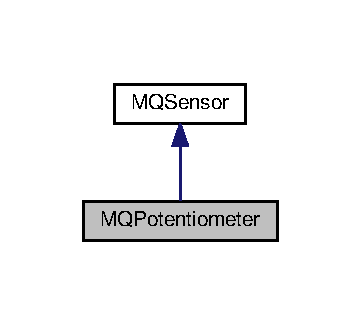
\includegraphics[width=173pt]{class_m_q_potentiometer__inherit__graph}
\end{center}
\end{figure}


Collaboration diagram for M\+Q\+Potentiometer\+:\nopagebreak
\begin{figure}[H]
\begin{center}
\leavevmode
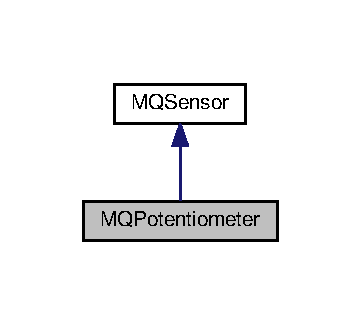
\includegraphics[width=173pt]{class_m_q_potentiometer__coll__graph}
\end{center}
\end{figure}
\subsection*{Public Member Functions}
\begin{DoxyCompactItemize}
\item 
\hyperlink{class_m_q_potentiometer_a9a890ae1eee63b533f2865fcc82a5e66}{M\+Q\+Potentiometer} (const uint8\+\_\+t mqpin)
\end{DoxyCompactItemize}
\subsection*{Additional Inherited Members}


\subsection{Detailed Description}
This uses a potentiometer as a sensor, to be used to generate values for debugging purposes. May be of better use if expandanded to handle a gas curve.

\begin{DoxyAuthor}{Author}
Daniel Pereira Poltronieri 
\end{DoxyAuthor}
\begin{DoxyDate}{Date}
October, 2017 Contact\+: \href{mailto:danppoltronieri@gmail.com}{\tt danppoltronieri@gmail.\+com} 
\end{DoxyDate}


Definition at line 150 of file M\+Q\+Sensor.\+hpp.



\subsection{Constructor \& Destructor Documentation}
\index{M\+Q\+Potentiometer@{M\+Q\+Potentiometer}!M\+Q\+Potentiometer@{M\+Q\+Potentiometer}}
\index{M\+Q\+Potentiometer@{M\+Q\+Potentiometer}!M\+Q\+Potentiometer@{M\+Q\+Potentiometer}}
\subsubsection[{\texorpdfstring{M\+Q\+Potentiometer(const uint8\+\_\+t mqpin)}{MQPotentiometer(const uint8_t mqpin)}}]{\setlength{\rightskip}{0pt plus 5cm}M\+Q\+Potentiometer\+::\+M\+Q\+Potentiometer (
\begin{DoxyParamCaption}
\item[{const uint8\+\_\+t}]{mqpin}
\end{DoxyParamCaption}
)}\hypertarget{class_m_q_potentiometer_a9a890ae1eee63b533f2865fcc82a5e66}{}\label{class_m_q_potentiometer_a9a890ae1eee63b533f2865fcc82a5e66}


Definition at line 270 of file M\+Q\+Sensor.\+cpp.



The documentation for this class was generated from the following files\+:\begin{DoxyCompactItemize}
\item 
lib/\+M\+Q-\/\+Sensor/src/\hyperlink{_m_q_sensor_8hpp}{M\+Q\+Sensor.\+hpp}\item 
lib/\+M\+Q-\/\+Sensor/src/\hyperlink{_m_q_sensor_8cpp}{M\+Q\+Sensor.\+cpp}\end{DoxyCompactItemize}

\hypertarget{class_m_q_sensor}{}\section{M\+Q\+Sensor Class Reference}
\label{class_m_q_sensor}\index{M\+Q\+Sensor@{M\+Q\+Sensor}}


{\ttfamily \#include $<$M\+Q\+Sensor.\+hpp$>$}



Inheritance diagram for M\+Q\+Sensor\+:
% FIG 0
\subsection*{Public Member Functions}
\begin{DoxyCompactItemize}
\item 
uint16\+\_\+t \hyperlink{class_m_q_sensor_acc2b495b544c2e801a4708c91df7a874}{check} (void)
\item 
void \hyperlink{class_m_q_sensor_ae6d1b0181e6769745caf5766ceef1522}{begin} ()
\item 
void \hyperlink{class_m_q_sensor_a54d01cd9465f177f431f070f7e96821d}{set\+Rl\+Value} (const uint8\+\_\+t rlvalue)
\item 
void \hyperlink{class_m_q_sensor_ad93e118f8bce230241af72307a7c2b79}{set\+Calibration\+Sample\+Times} (const uint8\+\_\+t cst)
\item 
void \hyperlink{class_m_q_sensor_ad14ad2558241aac29113e13b8a5137f7}{set\+Calibration\+Sample\+Interval} (const uint8\+\_\+t csi)
\item 
void \hyperlink{class_m_q_sensor_acefcf4fca770e50814f32bac2c80459c}{set\+Read\+Sample\+Interval} (const uint8\+\_\+t rsi)
\item 
void \hyperlink{class_m_q_sensor_a8e4a65e66a55f8abbe4365400e27ab97}{set\+Read\+Sample\+Times} (const uint8\+\_\+t rst)
\item 
void \hyperlink{class_m_q_sensor_a03eb97a82d462ee54ed249bc11da916a}{Set\+Ro} (const float ro\+\_\+factor)
\item 
void \hyperlink{class_m_q_sensor_a870f6dacc4896cdea8cb114b3b508ea3}{Set\+Ro\+Clean\+Air\+Factor} (const float ro\+\_\+clean\+\_\+air\+\_\+factor)
\item 
float const \hyperlink{class_m_q_sensor_a48389f7f5b5757092f7ae7a0893fe33f}{Get\+Ro\+Clean\+Air\+Factor} (void)
\item 
float const \hyperlink{class_m_q_sensor_a7292dbbdb30f7dac813f16009b6cd282}{Get\+Ro} (void)
\end{DoxyCompactItemize}
\subsection*{Static Public Member Functions}
\begin{DoxyCompactItemize}
\item 
static \hyperlink{class_m_q_sensor}{M\+Q\+Sensor} \hyperlink{class_m_q_sensor_a7f29aed48ad89d8403f08a4e83b136b5}{New\+M\+Q\+Sensor} (const uint8\+\_\+t mqpin, const uint8\+\_\+t mqtype)
\end{DoxyCompactItemize}
\subsection*{Protected Member Functions}
\begin{DoxyCompactItemize}
\item 
\hyperlink{class_m_q_sensor_a58bc8dbc8dc2e97584a34f1a545f93e1}{M\+Q\+Sensor} (const uint8\+\_\+t mqpin)
\item 
float const \hyperlink{class_m_q_sensor_ac769cc3eade7067313d185848f63f2cf}{M\+Q\+Read} ()
\item 
float const \hyperlink{class_m_q_sensor_a92ef594a160b257ca124481a21840a96}{M\+Q\+Get\+Percentage} (const float rs\+\_\+ro\+\_\+ratio, const float $\ast$pcurve)
\item 
float \hyperlink{class_m_q_sensor_aae67f9f2749712bd2afa90a2a97a29fd}{M\+Q\+Calibration} ()
\item 
float const \hyperlink{class_m_q_sensor_a1bb39a92869446ede5ba1c6854034e20}{M\+Q\+Resistance\+Calculation} (const int raw\+\_\+adc)
\end{DoxyCompactItemize}
\subsection*{Protected Attributes}
\begin{DoxyCompactItemize}
\item 
size\+\_\+t \hyperlink{class_m_q_sensor_a464b0db94d80b771efca70a0eb58f951}{\+\_\+\+L\+A\+S\+T\+\_\+\+R\+E\+A\+D\+\_\+\+T\+I\+ME} = 0
\item 
size\+\_\+t \hyperlink{class_m_q_sensor_a4a8e710f1bc61afb702d26ceb1366f11}{\+\_\+\+R\+E\+A\+D\+\_\+\+S\+E\+N\+S\+O\+R\+\_\+\+I\+N\+T\+E\+R\+V\+AL} = 10000
\item 
uint8\+\_\+t \hyperlink{class_m_q_sensor_aaa75c5a8dbb6b8bfba63a7b8749acd82}{\+\_\+\+M\+Q\+\_\+pin}
\item 
uint8\+\_\+t \hyperlink{class_m_q_sensor_ae04756d16f8d90e492fdb48c5ac4e930}{\+\_\+\+C\+A\+L\+I\+B\+A\+R\+A\+I\+O\+N\+\_\+\+S\+A\+M\+P\+L\+E\+\_\+\+T\+I\+M\+ES} = 5
\item 
uint8\+\_\+t \hyperlink{class_m_q_sensor_a440f40e2d8109c9cda26ce2b3d8ff564}{\+\_\+\+C\+A\+L\+I\+B\+R\+A\+T\+I\+O\+N\+\_\+\+S\+A\+M\+P\+L\+E\+\_\+\+I\+N\+T\+E\+R\+V\+AL} = 50
\item 
uint8\+\_\+t \hyperlink{class_m_q_sensor_a7dcb6e9f9ff88b498d7b47dd33b0809f}{\+\_\+\+R\+E\+A\+D\+\_\+\+S\+A\+M\+P\+L\+E\+\_\+\+I\+N\+T\+E\+R\+V\+AL} = 50
\item 
uint8\+\_\+t \hyperlink{class_m_q_sensor_a3c6ba8a07087b67ee99941bced73e940}{\+\_\+\+R\+E\+A\+D\+\_\+\+S\+A\+M\+P\+L\+E\+\_\+\+T\+I\+M\+ES} = 5
\item 
float \hyperlink{class_m_q_sensor_adc7e7af2139868a784d31d27d73b7df3}{\+\_\+\+R\+O\+\_\+\+C\+L\+E\+A\+N\+\_\+\+A\+I\+R\+\_\+\+F\+A\+C\+T\+OR} = 9.\+83
\item 
float \hyperlink{class_m_q_sensor_ade2e483ebc557d1caf753d41a8b3afde}{\+\_\+\+Ro} = 10
\item 
float \hyperlink{class_m_q_sensor_a2cf9585b95f5beaac2dc8edbab7eff42}{\+\_\+\+R\+L\+\_\+\+V\+A\+L\+UE} = 5
\end{DoxyCompactItemize}


\subsection{Detailed Description}


Definition at line 35 of file M\+Q\+Sensor.\+hpp.



\subsection{Constructor \& Destructor Documentation}
\index{M\+Q\+Sensor@{M\+Q\+Sensor}!M\+Q\+Sensor@{M\+Q\+Sensor}}
\index{M\+Q\+Sensor@{M\+Q\+Sensor}!M\+Q\+Sensor@{M\+Q\+Sensor}}
\subsubsection[{\texorpdfstring{M\+Q\+Sensor(const uint8\+\_\+t mqpin)}{MQSensor(const uint8_t mqpin)}}]{\setlength{\rightskip}{0pt plus 5cm}M\+Q\+Sensor\+::\+M\+Q\+Sensor (
\begin{DoxyParamCaption}
\item[{const uint8\+\_\+t}]{mqpin}
\end{DoxyParamCaption}
)\hspace{0.3cm}{\ttfamily [protected]}}\hypertarget{class_m_q_sensor_a58bc8dbc8dc2e97584a34f1a545f93e1}{}\label{class_m_q_sensor_a58bc8dbc8dc2e97584a34f1a545f93e1}


Definition at line 29 of file M\+Q\+Sensor.\+cpp.



\subsection{Member Function Documentation}
\index{M\+Q\+Sensor@{M\+Q\+Sensor}!begin@{begin}}
\index{begin@{begin}!M\+Q\+Sensor@{M\+Q\+Sensor}}
\subsubsection[{\texorpdfstring{begin()}{begin()}}]{\setlength{\rightskip}{0pt plus 5cm}void M\+Q\+Sensor\+::begin (
\begin{DoxyParamCaption}
{}
\end{DoxyParamCaption}
)}\hypertarget{class_m_q_sensor_ae6d1b0181e6769745caf5766ceef1522}{}\label{class_m_q_sensor_ae6d1b0181e6769745caf5766ceef1522}


Definition at line 75 of file M\+Q\+Sensor.\+cpp.



Here is the call graph for this function\+:
% FIG 1




Here is the caller graph for this function\+:
% FIG 2


\index{M\+Q\+Sensor@{M\+Q\+Sensor}!check@{check}}
\index{check@{check}!M\+Q\+Sensor@{M\+Q\+Sensor}}
\subsubsection[{\texorpdfstring{check(void)}{check(void)}}]{\setlength{\rightskip}{0pt plus 5cm}uint16\+\_\+t M\+Q\+Sensor\+::check (
\begin{DoxyParamCaption}
\item[{void}]{}
\end{DoxyParamCaption}
)\hspace{0.3cm}{\ttfamily [inline]}}\hypertarget{class_m_q_sensor_acc2b495b544c2e801a4708c91df7a874}{}\label{class_m_q_sensor_acc2b495b544c2e801a4708c91df7a874}


Definition at line 43 of file M\+Q\+Sensor.\+hpp.



Here is the call graph for this function\+:
% FIG 3




Here is the caller graph for this function\+:
% FIG 4


\index{M\+Q\+Sensor@{M\+Q\+Sensor}!Get\+Ro@{Get\+Ro}}
\index{Get\+Ro@{Get\+Ro}!M\+Q\+Sensor@{M\+Q\+Sensor}}
\subsubsection[{\texorpdfstring{Get\+Ro(void)}{GetRo(void)}}]{\setlength{\rightskip}{0pt plus 5cm}float const M\+Q\+Sensor\+::\+Get\+Ro (
\begin{DoxyParamCaption}
\item[{void}]{}
\end{DoxyParamCaption}
)}\hypertarget{class_m_q_sensor_a7292dbbdb30f7dac813f16009b6cd282}{}\label{class_m_q_sensor_a7292dbbdb30f7dac813f16009b6cd282}


Definition at line 70 of file M\+Q\+Sensor.\+cpp.



Here is the caller graph for this function\+:
% FIG 5


\index{M\+Q\+Sensor@{M\+Q\+Sensor}!Get\+Ro\+Clean\+Air\+Factor@{Get\+Ro\+Clean\+Air\+Factor}}
\index{Get\+Ro\+Clean\+Air\+Factor@{Get\+Ro\+Clean\+Air\+Factor}!M\+Q\+Sensor@{M\+Q\+Sensor}}
\subsubsection[{\texorpdfstring{Get\+Ro\+Clean\+Air\+Factor(void)}{GetRoCleanAirFactor(void)}}]{\setlength{\rightskip}{0pt plus 5cm}float const M\+Q\+Sensor\+::\+Get\+Ro\+Clean\+Air\+Factor (
\begin{DoxyParamCaption}
\item[{void}]{}
\end{DoxyParamCaption}
)}\hypertarget{class_m_q_sensor_a48389f7f5b5757092f7ae7a0893fe33f}{}\label{class_m_q_sensor_a48389f7f5b5757092f7ae7a0893fe33f}


Definition at line 67 of file M\+Q\+Sensor.\+cpp.



Here is the caller graph for this function\+:
% FIG 6


\index{M\+Q\+Sensor@{M\+Q\+Sensor}!M\+Q\+Calibration@{M\+Q\+Calibration}}
\index{M\+Q\+Calibration@{M\+Q\+Calibration}!M\+Q\+Sensor@{M\+Q\+Sensor}}
\subsubsection[{\texorpdfstring{M\+Q\+Calibration()}{MQCalibration()}}]{\setlength{\rightskip}{0pt plus 5cm}float M\+Q\+Sensor\+::\+M\+Q\+Calibration (
\begin{DoxyParamCaption}
{}
\end{DoxyParamCaption}
)\hspace{0.3cm}{\ttfamily [protected]}}\hypertarget{class_m_q_sensor_aae67f9f2749712bd2afa90a2a97a29fd}{}\label{class_m_q_sensor_aae67f9f2749712bd2afa90a2a97a29fd}


Definition at line 123 of file M\+Q\+Sensor.\+cpp.



Here is the call graph for this function\+:
% FIG 7




Here is the caller graph for this function\+:
% FIG 8


\index{M\+Q\+Sensor@{M\+Q\+Sensor}!M\+Q\+Get\+Percentage@{M\+Q\+Get\+Percentage}}
\index{M\+Q\+Get\+Percentage@{M\+Q\+Get\+Percentage}!M\+Q\+Sensor@{M\+Q\+Sensor}}
\subsubsection[{\texorpdfstring{M\+Q\+Get\+Percentage(const float rs\+\_\+ro\+\_\+ratio, const float $\ast$pcurve)}{MQGetPercentage(const float rs_ro_ratio, const float *pcurve)}}]{\setlength{\rightskip}{0pt plus 5cm}float const M\+Q\+Sensor\+::\+M\+Q\+Get\+Percentage (
\begin{DoxyParamCaption}
\item[{const float}]{rs\+\_\+ro\+\_\+ratio, }
\item[{const float $\ast$}]{pcurve}
\end{DoxyParamCaption}
)\hspace{0.3cm}{\ttfamily [protected]}}\hypertarget{class_m_q_sensor_a92ef594a160b257ca124481a21840a96}{}\label{class_m_q_sensor_a92ef594a160b257ca124481a21840a96}


Definition at line 161 of file M\+Q\+Sensor.\+cpp.



Here is the caller graph for this function\+:
% FIG 9


\index{M\+Q\+Sensor@{M\+Q\+Sensor}!M\+Q\+Read@{M\+Q\+Read}}
\index{M\+Q\+Read@{M\+Q\+Read}!M\+Q\+Sensor@{M\+Q\+Sensor}}
\subsubsection[{\texorpdfstring{M\+Q\+Read()}{MQRead()}}]{\setlength{\rightskip}{0pt plus 5cm}float const M\+Q\+Sensor\+::\+M\+Q\+Read (
\begin{DoxyParamCaption}
{}
\end{DoxyParamCaption}
)\hspace{0.3cm}{\ttfamily [protected]}}\hypertarget{class_m_q_sensor_ac769cc3eade7067313d185848f63f2cf}{}\label{class_m_q_sensor_ac769cc3eade7067313d185848f63f2cf}


Definition at line 138 of file M\+Q\+Sensor.\+cpp.



Here is the call graph for this function\+:
% FIG 10




Here is the caller graph for this function\+:
% FIG 11


\index{M\+Q\+Sensor@{M\+Q\+Sensor}!M\+Q\+Resistance\+Calculation@{M\+Q\+Resistance\+Calculation}}
\index{M\+Q\+Resistance\+Calculation@{M\+Q\+Resistance\+Calculation}!M\+Q\+Sensor@{M\+Q\+Sensor}}
\subsubsection[{\texorpdfstring{M\+Q\+Resistance\+Calculation(const int raw\+\_\+adc)}{MQResistanceCalculation(const int raw_adc)}}]{\setlength{\rightskip}{0pt plus 5cm}float const M\+Q\+Sensor\+::\+M\+Q\+Resistance\+Calculation (
\begin{DoxyParamCaption}
\item[{const int}]{raw\+\_\+adc}
\end{DoxyParamCaption}
)\hspace{0.3cm}{\ttfamily [inline]}, {\ttfamily [protected]}}\hypertarget{class_m_q_sensor_a1bb39a92869446ede5ba1c6854034e20}{}\label{class_m_q_sensor_a1bb39a92869446ede5ba1c6854034e20}


Definition at line 92 of file M\+Q\+Sensor.\+cpp.



Here is the caller graph for this function\+:
% FIG 12


\index{M\+Q\+Sensor@{M\+Q\+Sensor}!New\+M\+Q\+Sensor@{New\+M\+Q\+Sensor}}
\index{New\+M\+Q\+Sensor@{New\+M\+Q\+Sensor}!M\+Q\+Sensor@{M\+Q\+Sensor}}
\subsubsection[{\texorpdfstring{New\+M\+Q\+Sensor(const uint8\+\_\+t mqpin, const uint8\+\_\+t mqtype)}{NewMQSensor(const uint8_t mqpin, const uint8_t mqtype)}}]{\setlength{\rightskip}{0pt plus 5cm}{\bf M\+Q\+Sensor} M\+Q\+Sensor\+::\+New\+M\+Q\+Sensor (
\begin{DoxyParamCaption}
\item[{const uint8\+\_\+t}]{mqpin, }
\item[{const uint8\+\_\+t}]{mqtype}
\end{DoxyParamCaption}
)\hspace{0.3cm}{\ttfamily [static]}}\hypertarget{class_m_q_sensor_a7f29aed48ad89d8403f08a4e83b136b5}{}\label{class_m_q_sensor_a7f29aed48ad89d8403f08a4e83b136b5}


Definition at line 7 of file M\+Q\+Sensor.\+cpp.

\index{M\+Q\+Sensor@{M\+Q\+Sensor}!set\+Calibration\+Sample\+Interval@{set\+Calibration\+Sample\+Interval}}
\index{set\+Calibration\+Sample\+Interval@{set\+Calibration\+Sample\+Interval}!M\+Q\+Sensor@{M\+Q\+Sensor}}
\subsubsection[{\texorpdfstring{set\+Calibration\+Sample\+Interval(const uint8\+\_\+t csi)}{setCalibrationSampleInterval(const uint8_t csi)}}]{\setlength{\rightskip}{0pt plus 5cm}void M\+Q\+Sensor\+::set\+Calibration\+Sample\+Interval (
\begin{DoxyParamCaption}
\item[{const uint8\+\_\+t}]{csi}
\end{DoxyParamCaption}
)}\hypertarget{class_m_q_sensor_ad14ad2558241aac29113e13b8a5137f7}{}\label{class_m_q_sensor_ad14ad2558241aac29113e13b8a5137f7}


Definition at line 58 of file M\+Q\+Sensor.\+cpp.



Here is the caller graph for this function\+:
% FIG 13


\index{M\+Q\+Sensor@{M\+Q\+Sensor}!set\+Calibration\+Sample\+Times@{set\+Calibration\+Sample\+Times}}
\index{set\+Calibration\+Sample\+Times@{set\+Calibration\+Sample\+Times}!M\+Q\+Sensor@{M\+Q\+Sensor}}
\subsubsection[{\texorpdfstring{set\+Calibration\+Sample\+Times(const uint8\+\_\+t cst)}{setCalibrationSampleTimes(const uint8_t cst)}}]{\setlength{\rightskip}{0pt plus 5cm}void M\+Q\+Sensor\+::set\+Calibration\+Sample\+Times (
\begin{DoxyParamCaption}
\item[{const uint8\+\_\+t}]{cst}
\end{DoxyParamCaption}
)}\hypertarget{class_m_q_sensor_ad93e118f8bce230241af72307a7c2b79}{}\label{class_m_q_sensor_ad93e118f8bce230241af72307a7c2b79}


Definition at line 55 of file M\+Q\+Sensor.\+cpp.



Here is the caller graph for this function\+:
% FIG 14


\index{M\+Q\+Sensor@{M\+Q\+Sensor}!set\+Read\+Sample\+Interval@{set\+Read\+Sample\+Interval}}
\index{set\+Read\+Sample\+Interval@{set\+Read\+Sample\+Interval}!M\+Q\+Sensor@{M\+Q\+Sensor}}
\subsubsection[{\texorpdfstring{set\+Read\+Sample\+Interval(const uint8\+\_\+t rsi)}{setReadSampleInterval(const uint8_t rsi)}}]{\setlength{\rightskip}{0pt plus 5cm}void M\+Q\+Sensor\+::set\+Read\+Sample\+Interval (
\begin{DoxyParamCaption}
\item[{const uint8\+\_\+t}]{rsi}
\end{DoxyParamCaption}
)}\hypertarget{class_m_q_sensor_acefcf4fca770e50814f32bac2c80459c}{}\label{class_m_q_sensor_acefcf4fca770e50814f32bac2c80459c}


Definition at line 61 of file M\+Q\+Sensor.\+cpp.



Here is the caller graph for this function\+:
% FIG 15


\index{M\+Q\+Sensor@{M\+Q\+Sensor}!set\+Read\+Sample\+Times@{set\+Read\+Sample\+Times}}
\index{set\+Read\+Sample\+Times@{set\+Read\+Sample\+Times}!M\+Q\+Sensor@{M\+Q\+Sensor}}
\subsubsection[{\texorpdfstring{set\+Read\+Sample\+Times(const uint8\+\_\+t rst)}{setReadSampleTimes(const uint8_t rst)}}]{\setlength{\rightskip}{0pt plus 5cm}void M\+Q\+Sensor\+::set\+Read\+Sample\+Times (
\begin{DoxyParamCaption}
\item[{const uint8\+\_\+t}]{rst}
\end{DoxyParamCaption}
)}\hypertarget{class_m_q_sensor_a8e4a65e66a55f8abbe4365400e27ab97}{}\label{class_m_q_sensor_a8e4a65e66a55f8abbe4365400e27ab97}


Definition at line 64 of file M\+Q\+Sensor.\+cpp.



Here is the caller graph for this function\+:
% FIG 16


\index{M\+Q\+Sensor@{M\+Q\+Sensor}!set\+Rl\+Value@{set\+Rl\+Value}}
\index{set\+Rl\+Value@{set\+Rl\+Value}!M\+Q\+Sensor@{M\+Q\+Sensor}}
\subsubsection[{\texorpdfstring{set\+Rl\+Value(const uint8\+\_\+t rlvalue)}{setRlValue(const uint8_t rlvalue)}}]{\setlength{\rightskip}{0pt plus 5cm}void M\+Q\+Sensor\+::set\+Rl\+Value (
\begin{DoxyParamCaption}
\item[{const uint8\+\_\+t}]{rlvalue}
\end{DoxyParamCaption}
)}\hypertarget{class_m_q_sensor_a54d01cd9465f177f431f070f7e96821d}{}\label{class_m_q_sensor_a54d01cd9465f177f431f070f7e96821d}


Definition at line 52 of file M\+Q\+Sensor.\+cpp.



Here is the caller graph for this function\+:
% FIG 17


\index{M\+Q\+Sensor@{M\+Q\+Sensor}!Set\+Ro@{Set\+Ro}}
\index{Set\+Ro@{Set\+Ro}!M\+Q\+Sensor@{M\+Q\+Sensor}}
\subsubsection[{\texorpdfstring{Set\+Ro(const float ro\+\_\+factor)}{SetRo(const float ro_factor)}}]{\setlength{\rightskip}{0pt plus 5cm}void M\+Q\+Sensor\+::\+Set\+Ro (
\begin{DoxyParamCaption}
\item[{const float}]{ro\+\_\+factor}
\end{DoxyParamCaption}
)}\hypertarget{class_m_q_sensor_a03eb97a82d462ee54ed249bc11da916a}{}\label{class_m_q_sensor_a03eb97a82d462ee54ed249bc11da916a}


Definition at line 46 of file M\+Q\+Sensor.\+cpp.



Here is the caller graph for this function\+:
% FIG 18


\index{M\+Q\+Sensor@{M\+Q\+Sensor}!Set\+Ro\+Clean\+Air\+Factor@{Set\+Ro\+Clean\+Air\+Factor}}
\index{Set\+Ro\+Clean\+Air\+Factor@{Set\+Ro\+Clean\+Air\+Factor}!M\+Q\+Sensor@{M\+Q\+Sensor}}
\subsubsection[{\texorpdfstring{Set\+Ro\+Clean\+Air\+Factor(const float ro\+\_\+clean\+\_\+air\+\_\+factor)}{SetRoCleanAirFactor(const float ro_clean_air_factor)}}]{\setlength{\rightskip}{0pt plus 5cm}void M\+Q\+Sensor\+::\+Set\+Ro\+Clean\+Air\+Factor (
\begin{DoxyParamCaption}
\item[{const float}]{ro\+\_\+clean\+\_\+air\+\_\+factor}
\end{DoxyParamCaption}
)}\hypertarget{class_m_q_sensor_a870f6dacc4896cdea8cb114b3b508ea3}{}\label{class_m_q_sensor_a870f6dacc4896cdea8cb114b3b508ea3}


Definition at line 49 of file M\+Q\+Sensor.\+cpp.



Here is the caller graph for this function\+:
% FIG 19




\subsection{Member Data Documentation}
\index{M\+Q\+Sensor@{M\+Q\+Sensor}!\+\_\+\+C\+A\+L\+I\+B\+A\+R\+A\+I\+O\+N\+\_\+\+S\+A\+M\+P\+L\+E\+\_\+\+T\+I\+M\+ES@{\+\_\+\+C\+A\+L\+I\+B\+A\+R\+A\+I\+O\+N\+\_\+\+S\+A\+M\+P\+L\+E\+\_\+\+T\+I\+M\+ES}}
\index{\+\_\+\+C\+A\+L\+I\+B\+A\+R\+A\+I\+O\+N\+\_\+\+S\+A\+M\+P\+L\+E\+\_\+\+T\+I\+M\+ES@{\+\_\+\+C\+A\+L\+I\+B\+A\+R\+A\+I\+O\+N\+\_\+\+S\+A\+M\+P\+L\+E\+\_\+\+T\+I\+M\+ES}!M\+Q\+Sensor@{M\+Q\+Sensor}}
\subsubsection[{\texorpdfstring{\+\_\+\+C\+A\+L\+I\+B\+A\+R\+A\+I\+O\+N\+\_\+\+S\+A\+M\+P\+L\+E\+\_\+\+T\+I\+M\+ES}{_CALIBARAION_SAMPLE_TIMES}}]{\setlength{\rightskip}{0pt plus 5cm}uint8\+\_\+t M\+Q\+Sensor\+::\+\_\+\+C\+A\+L\+I\+B\+A\+R\+A\+I\+O\+N\+\_\+\+S\+A\+M\+P\+L\+E\+\_\+\+T\+I\+M\+ES = 5\hspace{0.3cm}{\ttfamily [protected]}}\hypertarget{class_m_q_sensor_ae04756d16f8d90e492fdb48c5ac4e930}{}\label{class_m_q_sensor_ae04756d16f8d90e492fdb48c5ac4e930}


Definition at line 67 of file M\+Q\+Sensor.\+hpp.

\index{M\+Q\+Sensor@{M\+Q\+Sensor}!\+\_\+\+C\+A\+L\+I\+B\+R\+A\+T\+I\+O\+N\+\_\+\+S\+A\+M\+P\+L\+E\+\_\+\+I\+N\+T\+E\+R\+V\+AL@{\+\_\+\+C\+A\+L\+I\+B\+R\+A\+T\+I\+O\+N\+\_\+\+S\+A\+M\+P\+L\+E\+\_\+\+I\+N\+T\+E\+R\+V\+AL}}
\index{\+\_\+\+C\+A\+L\+I\+B\+R\+A\+T\+I\+O\+N\+\_\+\+S\+A\+M\+P\+L\+E\+\_\+\+I\+N\+T\+E\+R\+V\+AL@{\+\_\+\+C\+A\+L\+I\+B\+R\+A\+T\+I\+O\+N\+\_\+\+S\+A\+M\+P\+L\+E\+\_\+\+I\+N\+T\+E\+R\+V\+AL}!M\+Q\+Sensor@{M\+Q\+Sensor}}
\subsubsection[{\texorpdfstring{\+\_\+\+C\+A\+L\+I\+B\+R\+A\+T\+I\+O\+N\+\_\+\+S\+A\+M\+P\+L\+E\+\_\+\+I\+N\+T\+E\+R\+V\+AL}{_CALIBRATION_SAMPLE_INTERVAL}}]{\setlength{\rightskip}{0pt plus 5cm}uint8\+\_\+t M\+Q\+Sensor\+::\+\_\+\+C\+A\+L\+I\+B\+R\+A\+T\+I\+O\+N\+\_\+\+S\+A\+M\+P\+L\+E\+\_\+\+I\+N\+T\+E\+R\+V\+AL = 50\hspace{0.3cm}{\ttfamily [protected]}}\hypertarget{class_m_q_sensor_a440f40e2d8109c9cda26ce2b3d8ff564}{}\label{class_m_q_sensor_a440f40e2d8109c9cda26ce2b3d8ff564}


Definition at line 68 of file M\+Q\+Sensor.\+hpp.

\index{M\+Q\+Sensor@{M\+Q\+Sensor}!\+\_\+\+L\+A\+S\+T\+\_\+\+R\+E\+A\+D\+\_\+\+T\+I\+ME@{\+\_\+\+L\+A\+S\+T\+\_\+\+R\+E\+A\+D\+\_\+\+T\+I\+ME}}
\index{\+\_\+\+L\+A\+S\+T\+\_\+\+R\+E\+A\+D\+\_\+\+T\+I\+ME@{\+\_\+\+L\+A\+S\+T\+\_\+\+R\+E\+A\+D\+\_\+\+T\+I\+ME}!M\+Q\+Sensor@{M\+Q\+Sensor}}
\subsubsection[{\texorpdfstring{\+\_\+\+L\+A\+S\+T\+\_\+\+R\+E\+A\+D\+\_\+\+T\+I\+ME}{_LAST_READ_TIME}}]{\setlength{\rightskip}{0pt plus 5cm}size\+\_\+t M\+Q\+Sensor\+::\+\_\+\+L\+A\+S\+T\+\_\+\+R\+E\+A\+D\+\_\+\+T\+I\+ME = 0\hspace{0.3cm}{\ttfamily [protected]}}\hypertarget{class_m_q_sensor_a464b0db94d80b771efca70a0eb58f951}{}\label{class_m_q_sensor_a464b0db94d80b771efca70a0eb58f951}


Definition at line 64 of file M\+Q\+Sensor.\+hpp.

\index{M\+Q\+Sensor@{M\+Q\+Sensor}!\+\_\+\+M\+Q\+\_\+pin@{\+\_\+\+M\+Q\+\_\+pin}}
\index{\+\_\+\+M\+Q\+\_\+pin@{\+\_\+\+M\+Q\+\_\+pin}!M\+Q\+Sensor@{M\+Q\+Sensor}}
\subsubsection[{\texorpdfstring{\+\_\+\+M\+Q\+\_\+pin}{_MQ_pin}}]{\setlength{\rightskip}{0pt plus 5cm}uint8\+\_\+t M\+Q\+Sensor\+::\+\_\+\+M\+Q\+\_\+pin\hspace{0.3cm}{\ttfamily [protected]}}\hypertarget{class_m_q_sensor_aaa75c5a8dbb6b8bfba63a7b8749acd82}{}\label{class_m_q_sensor_aaa75c5a8dbb6b8bfba63a7b8749acd82}


Definition at line 66 of file M\+Q\+Sensor.\+hpp.

\index{M\+Q\+Sensor@{M\+Q\+Sensor}!\+\_\+\+R\+E\+A\+D\+\_\+\+S\+A\+M\+P\+L\+E\+\_\+\+I\+N\+T\+E\+R\+V\+AL@{\+\_\+\+R\+E\+A\+D\+\_\+\+S\+A\+M\+P\+L\+E\+\_\+\+I\+N\+T\+E\+R\+V\+AL}}
\index{\+\_\+\+R\+E\+A\+D\+\_\+\+S\+A\+M\+P\+L\+E\+\_\+\+I\+N\+T\+E\+R\+V\+AL@{\+\_\+\+R\+E\+A\+D\+\_\+\+S\+A\+M\+P\+L\+E\+\_\+\+I\+N\+T\+E\+R\+V\+AL}!M\+Q\+Sensor@{M\+Q\+Sensor}}
\subsubsection[{\texorpdfstring{\+\_\+\+R\+E\+A\+D\+\_\+\+S\+A\+M\+P\+L\+E\+\_\+\+I\+N\+T\+E\+R\+V\+AL}{_READ_SAMPLE_INTERVAL}}]{\setlength{\rightskip}{0pt plus 5cm}uint8\+\_\+t M\+Q\+Sensor\+::\+\_\+\+R\+E\+A\+D\+\_\+\+S\+A\+M\+P\+L\+E\+\_\+\+I\+N\+T\+E\+R\+V\+AL = 50\hspace{0.3cm}{\ttfamily [protected]}}\hypertarget{class_m_q_sensor_a7dcb6e9f9ff88b498d7b47dd33b0809f}{}\label{class_m_q_sensor_a7dcb6e9f9ff88b498d7b47dd33b0809f}


Definition at line 69 of file M\+Q\+Sensor.\+hpp.

\index{M\+Q\+Sensor@{M\+Q\+Sensor}!\+\_\+\+R\+E\+A\+D\+\_\+\+S\+A\+M\+P\+L\+E\+\_\+\+T\+I\+M\+ES@{\+\_\+\+R\+E\+A\+D\+\_\+\+S\+A\+M\+P\+L\+E\+\_\+\+T\+I\+M\+ES}}
\index{\+\_\+\+R\+E\+A\+D\+\_\+\+S\+A\+M\+P\+L\+E\+\_\+\+T\+I\+M\+ES@{\+\_\+\+R\+E\+A\+D\+\_\+\+S\+A\+M\+P\+L\+E\+\_\+\+T\+I\+M\+ES}!M\+Q\+Sensor@{M\+Q\+Sensor}}
\subsubsection[{\texorpdfstring{\+\_\+\+R\+E\+A\+D\+\_\+\+S\+A\+M\+P\+L\+E\+\_\+\+T\+I\+M\+ES}{_READ_SAMPLE_TIMES}}]{\setlength{\rightskip}{0pt plus 5cm}uint8\+\_\+t M\+Q\+Sensor\+::\+\_\+\+R\+E\+A\+D\+\_\+\+S\+A\+M\+P\+L\+E\+\_\+\+T\+I\+M\+ES = 5\hspace{0.3cm}{\ttfamily [protected]}}\hypertarget{class_m_q_sensor_a3c6ba8a07087b67ee99941bced73e940}{}\label{class_m_q_sensor_a3c6ba8a07087b67ee99941bced73e940}


Definition at line 70 of file M\+Q\+Sensor.\+hpp.

\index{M\+Q\+Sensor@{M\+Q\+Sensor}!\+\_\+\+R\+E\+A\+D\+\_\+\+S\+E\+N\+S\+O\+R\+\_\+\+I\+N\+T\+E\+R\+V\+AL@{\+\_\+\+R\+E\+A\+D\+\_\+\+S\+E\+N\+S\+O\+R\+\_\+\+I\+N\+T\+E\+R\+V\+AL}}
\index{\+\_\+\+R\+E\+A\+D\+\_\+\+S\+E\+N\+S\+O\+R\+\_\+\+I\+N\+T\+E\+R\+V\+AL@{\+\_\+\+R\+E\+A\+D\+\_\+\+S\+E\+N\+S\+O\+R\+\_\+\+I\+N\+T\+E\+R\+V\+AL}!M\+Q\+Sensor@{M\+Q\+Sensor}}
\subsubsection[{\texorpdfstring{\+\_\+\+R\+E\+A\+D\+\_\+\+S\+E\+N\+S\+O\+R\+\_\+\+I\+N\+T\+E\+R\+V\+AL}{_READ_SENSOR_INTERVAL}}]{\setlength{\rightskip}{0pt plus 5cm}size\+\_\+t M\+Q\+Sensor\+::\+\_\+\+R\+E\+A\+D\+\_\+\+S\+E\+N\+S\+O\+R\+\_\+\+I\+N\+T\+E\+R\+V\+AL = 10000\hspace{0.3cm}{\ttfamily [protected]}}\hypertarget{class_m_q_sensor_a4a8e710f1bc61afb702d26ceb1366f11}{}\label{class_m_q_sensor_a4a8e710f1bc61afb702d26ceb1366f11}


Definition at line 65 of file M\+Q\+Sensor.\+hpp.

\index{M\+Q\+Sensor@{M\+Q\+Sensor}!\+\_\+\+R\+L\+\_\+\+V\+A\+L\+UE@{\+\_\+\+R\+L\+\_\+\+V\+A\+L\+UE}}
\index{\+\_\+\+R\+L\+\_\+\+V\+A\+L\+UE@{\+\_\+\+R\+L\+\_\+\+V\+A\+L\+UE}!M\+Q\+Sensor@{M\+Q\+Sensor}}
\subsubsection[{\texorpdfstring{\+\_\+\+R\+L\+\_\+\+V\+A\+L\+UE}{_RL_VALUE}}]{\setlength{\rightskip}{0pt plus 5cm}float M\+Q\+Sensor\+::\+\_\+\+R\+L\+\_\+\+V\+A\+L\+UE = 5\hspace{0.3cm}{\ttfamily [protected]}}\hypertarget{class_m_q_sensor_a2cf9585b95f5beaac2dc8edbab7eff42}{}\label{class_m_q_sensor_a2cf9585b95f5beaac2dc8edbab7eff42}


Definition at line 74 of file M\+Q\+Sensor.\+hpp.

\index{M\+Q\+Sensor@{M\+Q\+Sensor}!\+\_\+\+Ro@{\+\_\+\+Ro}}
\index{\+\_\+\+Ro@{\+\_\+\+Ro}!M\+Q\+Sensor@{M\+Q\+Sensor}}
\subsubsection[{\texorpdfstring{\+\_\+\+Ro}{_Ro}}]{\setlength{\rightskip}{0pt plus 5cm}float M\+Q\+Sensor\+::\+\_\+\+Ro = 10\hspace{0.3cm}{\ttfamily [protected]}}\hypertarget{class_m_q_sensor_ade2e483ebc557d1caf753d41a8b3afde}{}\label{class_m_q_sensor_ade2e483ebc557d1caf753d41a8b3afde}


Definition at line 73 of file M\+Q\+Sensor.\+hpp.

\index{M\+Q\+Sensor@{M\+Q\+Sensor}!\+\_\+\+R\+O\+\_\+\+C\+L\+E\+A\+N\+\_\+\+A\+I\+R\+\_\+\+F\+A\+C\+T\+OR@{\+\_\+\+R\+O\+\_\+\+C\+L\+E\+A\+N\+\_\+\+A\+I\+R\+\_\+\+F\+A\+C\+T\+OR}}
\index{\+\_\+\+R\+O\+\_\+\+C\+L\+E\+A\+N\+\_\+\+A\+I\+R\+\_\+\+F\+A\+C\+T\+OR@{\+\_\+\+R\+O\+\_\+\+C\+L\+E\+A\+N\+\_\+\+A\+I\+R\+\_\+\+F\+A\+C\+T\+OR}!M\+Q\+Sensor@{M\+Q\+Sensor}}
\subsubsection[{\texorpdfstring{\+\_\+\+R\+O\+\_\+\+C\+L\+E\+A\+N\+\_\+\+A\+I\+R\+\_\+\+F\+A\+C\+T\+OR}{_RO_CLEAN_AIR_FACTOR}}]{\setlength{\rightskip}{0pt plus 5cm}float M\+Q\+Sensor\+::\+\_\+\+R\+O\+\_\+\+C\+L\+E\+A\+N\+\_\+\+A\+I\+R\+\_\+\+F\+A\+C\+T\+OR = 9.\+83\hspace{0.3cm}{\ttfamily [protected]}}\hypertarget{class_m_q_sensor_adc7e7af2139868a784d31d27d73b7df3}{}\label{class_m_q_sensor_adc7e7af2139868a784d31d27d73b7df3}


Definition at line 72 of file M\+Q\+Sensor.\+hpp.



The documentation for this class was generated from the following files\+:\begin{DoxyCompactItemize}
\item 
lib/\+M\+Q-\/\+Sensor/src/\hyperlink{_m_q_sensor_8hpp}{M\+Q\+Sensor.\+hpp}\item 
lib/\+M\+Q-\/\+Sensor/src/\hyperlink{_m_q_sensor_8cpp}{M\+Q\+Sensor.\+cpp}\end{DoxyCompactItemize}

\hypertarget{class_print_manager}{}\section{Print\+Manager Class Reference}
\label{class_print_manager}\index{Print\+Manager@{Print\+Manager}}


{\ttfamily \#include $<$Print\+Manager.\+hpp$>$}



Collaboration diagram for Print\+Manager\+:\nopagebreak
\begin{figure}[H]
\begin{center}
\leavevmode
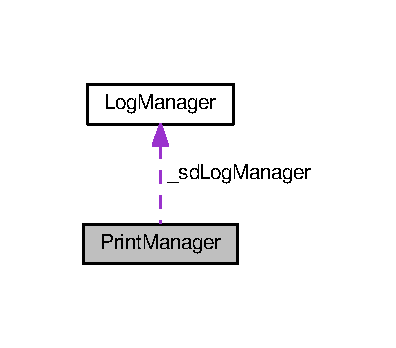
\includegraphics[width=190pt]{class_print_manager__coll__graph}
\end{center}
\end{figure}
\subsection*{Public Member Functions}
\begin{DoxyCompactItemize}
\item 
\hyperlink{class_print_manager_a587a22b1cc67696f71f5a85bfb130140}{Print\+Manager} (Hardware\+Serial $\ast$serial\+Port\+HW)
\item 
\hyperlink{class_print_manager_ac1212bb44b3c100bd67041d878977058}{Print\+Manager} (Software\+Serial $\ast$serial\+Port\+SW)
\item 
\hyperlink{class_print_manager_a5ac22dd7ed0f35b12cd2b7650e2c8501}{Print\+Manager} (Hardware\+Serial $\ast$serial\+Port\+HW, \hyperlink{class_log_manager}{Log\+Manager} $\ast$sd\+Log\+Manager)
\item 
\hyperlink{class_print_manager_ac1a82b54cdeaf43b3e78ed6eb18c9bc6}{Print\+Manager} (Software\+Serial $\ast$serial\+Port\+SW, \hyperlink{class_log_manager}{Log\+Manager} $\ast$sd\+Log\+Manager)
\item 
uint8\+\_\+t \hyperlink{class_print_manager_a65b6e94eb17c08725d307293c26922c6}{send\+Data} ()
\item 
void \hyperlink{class_print_manager_aef5dd6437e06e84de5a98c1466f5f074}{fast\+Value} (const char fmt, const double value)
\item 
void \hyperlink{class_print_manager_a27ea0c1977a54e1291d0be0fc0754f48}{add\+Value} (const char $\ast$fmt,...)
\item 
void \hyperlink{class_print_manager_a9a44c89a9752e1e1f63bc174ce675f90}{add\+Header} (const char $\ast$fmt,...)
\item 
void \hyperlink{class_print_manager_ae091788c5f4baa9df10fb290c67cb693}{fast\+Value} (const char $\ast$fmt,...)
\end{DoxyCompactItemize}
\subsection*{Protected Member Functions}
\begin{DoxyCompactItemize}
\item 
void \hyperlink{class_print_manager_abe73e179fbf7817ac2501663086efa6a}{make\+Header} ()
\item 
void \hyperlink{class_print_manager_aefa604ff2567aefd703c584cf530f581}{make\+Currently} ()
\end{DoxyCompactItemize}
\subsection*{Protected Attributes}
\begin{DoxyCompactItemize}
\item 
String \hyperlink{class_print_manager_a352c21440d4b8da910822603bbc6439d}{\+\_\+message\+Header} = \char`\"{}\{\char`\"{}
\item 
String \hyperlink{class_print_manager_a45a45bb347196bab8c3071cc5de6631a}{\+\_\+message\+Currently} = \char`\"{}\textbackslash{}\char`\"{}currently\textbackslash{}\char`\"{}\+: \{\char`\"{}
\item 
String \hyperlink{class_print_manager_ac499e04d25e84c7d7841d24c38a3bd47}{\+\_\+timezone} = \char`\"{}\textbackslash{}\char`\"{}Brazil/Brasília\textbackslash{}\char`\"{}\char`\"{}
\item 
uint8\+\_\+t \hyperlink{class_print_manager_ae1b8f767b738748027e0ac2a97f1be6c}{\+\_\+serial\+Port\+Type}
\item 
double \hyperlink{class_print_manager_a550ad6ba340af9c4f689b8e25bd420f3}{\+\_\+temp\+Value}
\item 
double \hyperlink{class_print_manager_a722d74baa1b0286c84b6d5181996ba2e}{\+\_\+latitude}
\item 
double \hyperlink{class_print_manager_a31a2a77dba86f3d99af5c6bd1d2baa4c}{\+\_\+longitude}
\item 
Hardware\+Serial $\ast$ \hyperlink{class_print_manager_a19cd58c07357e6142b92ed4598cda1bc}{\+\_\+serial\+Port\+HW}
\item 
Software\+Serial $\ast$ \hyperlink{class_print_manager_aa079f14838d51ffd18ac814323c3d177}{\+\_\+serial\+Port\+SW}
\item 
\hyperlink{class_log_manager}{Log\+Manager} $\ast$ \hyperlink{class_print_manager_a76f3172298d67da7428e55b2515aa030}{\+\_\+sd\+Log\+Manager}
\end{DoxyCompactItemize}


\subsection{Detailed Description}


Definition at line 15 of file Print\+Manager.\+hpp.



\subsection{Constructor \& Destructor Documentation}
\index{Print\+Manager@{Print\+Manager}!Print\+Manager@{Print\+Manager}}
\index{Print\+Manager@{Print\+Manager}!Print\+Manager@{Print\+Manager}}
\subsubsection[{\texorpdfstring{Print\+Manager(\+Hardware\+Serial $\ast$serial\+Port\+H\+W)}{PrintManager(HardwareSerial *serialPortHW)}}]{\setlength{\rightskip}{0pt plus 5cm}Print\+Manager\+::\+Print\+Manager (
\begin{DoxyParamCaption}
\item[{Hardware\+Serial $\ast$}]{serial\+Port\+HW}
\end{DoxyParamCaption}
)\hspace{0.3cm}{\ttfamily [inline]}}\hypertarget{class_print_manager_a587a22b1cc67696f71f5a85bfb130140}{}\label{class_print_manager_a587a22b1cc67696f71f5a85bfb130140}


Definition at line 17 of file Print\+Manager.\+hpp.

\index{Print\+Manager@{Print\+Manager}!Print\+Manager@{Print\+Manager}}
\index{Print\+Manager@{Print\+Manager}!Print\+Manager@{Print\+Manager}}
\subsubsection[{\texorpdfstring{Print\+Manager(\+Software\+Serial $\ast$serial\+Port\+S\+W)}{PrintManager(SoftwareSerial *serialPortSW)}}]{\setlength{\rightskip}{0pt plus 5cm}Print\+Manager\+::\+Print\+Manager (
\begin{DoxyParamCaption}
\item[{Software\+Serial $\ast$}]{serial\+Port\+SW}
\end{DoxyParamCaption}
)\hspace{0.3cm}{\ttfamily [inline]}}\hypertarget{class_print_manager_ac1212bb44b3c100bd67041d878977058}{}\label{class_print_manager_ac1212bb44b3c100bd67041d878977058}


Definition at line 23 of file Print\+Manager.\+hpp.

\index{Print\+Manager@{Print\+Manager}!Print\+Manager@{Print\+Manager}}
\index{Print\+Manager@{Print\+Manager}!Print\+Manager@{Print\+Manager}}
\subsubsection[{\texorpdfstring{Print\+Manager(\+Hardware\+Serial $\ast$serial\+Port\+H\+W, Log\+Manager $\ast$sd\+Log\+Manager)}{PrintManager(HardwareSerial *serialPortHW, LogManager *sdLogManager)}}]{\setlength{\rightskip}{0pt plus 5cm}Print\+Manager\+::\+Print\+Manager (
\begin{DoxyParamCaption}
\item[{Hardware\+Serial $\ast$}]{serial\+Port\+HW, }
\item[{{\bf Log\+Manager} $\ast$}]{sd\+Log\+Manager}
\end{DoxyParamCaption}
)\hspace{0.3cm}{\ttfamily [inline]}}\hypertarget{class_print_manager_a5ac22dd7ed0f35b12cd2b7650e2c8501}{}\label{class_print_manager_a5ac22dd7ed0f35b12cd2b7650e2c8501}


Definition at line 29 of file Print\+Manager.\+hpp.

\index{Print\+Manager@{Print\+Manager}!Print\+Manager@{Print\+Manager}}
\index{Print\+Manager@{Print\+Manager}!Print\+Manager@{Print\+Manager}}
\subsubsection[{\texorpdfstring{Print\+Manager(\+Software\+Serial $\ast$serial\+Port\+S\+W, Log\+Manager $\ast$sd\+Log\+Manager)}{PrintManager(SoftwareSerial *serialPortSW, LogManager *sdLogManager)}}]{\setlength{\rightskip}{0pt plus 5cm}Print\+Manager\+::\+Print\+Manager (
\begin{DoxyParamCaption}
\item[{Software\+Serial $\ast$}]{serial\+Port\+SW, }
\item[{{\bf Log\+Manager} $\ast$}]{sd\+Log\+Manager}
\end{DoxyParamCaption}
)\hspace{0.3cm}{\ttfamily [inline]}}\hypertarget{class_print_manager_ac1a82b54cdeaf43b3e78ed6eb18c9bc6}{}\label{class_print_manager_ac1a82b54cdeaf43b3e78ed6eb18c9bc6}


Definition at line 35 of file Print\+Manager.\+hpp.



\subsection{Member Function Documentation}
\index{Print\+Manager@{Print\+Manager}!add\+Header@{add\+Header}}
\index{add\+Header@{add\+Header}!Print\+Manager@{Print\+Manager}}
\subsubsection[{\texorpdfstring{add\+Header(const char $\ast$fmt,...)}{addHeader(const char *fmt,...)}}]{\setlength{\rightskip}{0pt plus 5cm}void Print\+Manager\+::add\+Header (
\begin{DoxyParamCaption}
\item[{const char $\ast$}]{fmt, }
\item[{}]{...}
\end{DoxyParamCaption}
)}\hypertarget{class_print_manager_a9a44c89a9752e1e1f63bc174ce675f90}{}\label{class_print_manager_a9a44c89a9752e1e1f63bc174ce675f90}


Definition at line 95 of file Print\+Manager.\+cpp.

\index{Print\+Manager@{Print\+Manager}!add\+Value@{add\+Value}}
\index{add\+Value@{add\+Value}!Print\+Manager@{Print\+Manager}}
\subsubsection[{\texorpdfstring{add\+Value(const char $\ast$fmt,...)}{addValue(const char *fmt,...)}}]{\setlength{\rightskip}{0pt plus 5cm}void Print\+Manager\+::add\+Value (
\begin{DoxyParamCaption}
\item[{const char $\ast$}]{fmt, }
\item[{}]{...}
\end{DoxyParamCaption}
)}\hypertarget{class_print_manager_a27ea0c1977a54e1291d0be0fc0754f48}{}\label{class_print_manager_a27ea0c1977a54e1291d0be0fc0754f48}


Definition at line 8 of file Print\+Manager.\+cpp.

\index{Print\+Manager@{Print\+Manager}!fast\+Value@{fast\+Value}}
\index{fast\+Value@{fast\+Value}!Print\+Manager@{Print\+Manager}}
\subsubsection[{\texorpdfstring{fast\+Value(const char fmt, const double value)}{fastValue(const char fmt, const double value)}}]{\setlength{\rightskip}{0pt plus 5cm}void Print\+Manager\+::fast\+Value (
\begin{DoxyParamCaption}
\item[{const char}]{fmt, }
\item[{const double}]{value}
\end{DoxyParamCaption}
)}\hypertarget{class_print_manager_aef5dd6437e06e84de5a98c1466f5f074}{}\label{class_print_manager_aef5dd6437e06e84de5a98c1466f5f074}


Definition at line 131 of file Print\+Manager.\+cpp.

\index{Print\+Manager@{Print\+Manager}!fast\+Value@{fast\+Value}}
\index{fast\+Value@{fast\+Value}!Print\+Manager@{Print\+Manager}}
\subsubsection[{\texorpdfstring{fast\+Value(const char $\ast$fmt,...)}{fastValue(const char *fmt,...)}}]{\setlength{\rightskip}{0pt plus 5cm}void Print\+Manager\+::fast\+Value (
\begin{DoxyParamCaption}
\item[{const char $\ast$}]{fmt, }
\item[{}]{...}
\end{DoxyParamCaption}
)}\hypertarget{class_print_manager_ae091788c5f4baa9df10fb290c67cb693}{}\label{class_print_manager_ae091788c5f4baa9df10fb290c67cb693}
\index{Print\+Manager@{Print\+Manager}!make\+Currently@{make\+Currently}}
\index{make\+Currently@{make\+Currently}!Print\+Manager@{Print\+Manager}}
\subsubsection[{\texorpdfstring{make\+Currently()}{makeCurrently()}}]{\setlength{\rightskip}{0pt plus 5cm}void Print\+Manager\+::make\+Currently (
\begin{DoxyParamCaption}
\item[{void}]{}
\end{DoxyParamCaption}
)\hspace{0.3cm}{\ttfamily [protected]}}\hypertarget{class_print_manager_aefa604ff2567aefd703c584cf530f581}{}\label{class_print_manager_aefa604ff2567aefd703c584cf530f581}


Definition at line 126 of file Print\+Manager.\+cpp.

\index{Print\+Manager@{Print\+Manager}!make\+Header@{make\+Header}}
\index{make\+Header@{make\+Header}!Print\+Manager@{Print\+Manager}}
\subsubsection[{\texorpdfstring{make\+Header()}{makeHeader()}}]{\setlength{\rightskip}{0pt plus 5cm}void Print\+Manager\+::make\+Header (
\begin{DoxyParamCaption}
\item[{void}]{}
\end{DoxyParamCaption}
)\hspace{0.3cm}{\ttfamily [protected]}}\hypertarget{class_print_manager_abe73e179fbf7817ac2501663086efa6a}{}\label{class_print_manager_abe73e179fbf7817ac2501663086efa6a}


Definition at line 116 of file Print\+Manager.\+cpp.

\index{Print\+Manager@{Print\+Manager}!send\+Data@{send\+Data}}
\index{send\+Data@{send\+Data}!Print\+Manager@{Print\+Manager}}
\subsubsection[{\texorpdfstring{send\+Data()}{sendData()}}]{\setlength{\rightskip}{0pt plus 5cm}uint8\+\_\+t Print\+Manager\+::send\+Data (
\begin{DoxyParamCaption}
{}
\end{DoxyParamCaption}
)}\hypertarget{class_print_manager_a65b6e94eb17c08725d307293c26922c6}{}\label{class_print_manager_a65b6e94eb17c08725d307293c26922c6}


Definition at line 137 of file Print\+Manager.\+cpp.



\subsection{Member Data Documentation}
\index{Print\+Manager@{Print\+Manager}!\+\_\+latitude@{\+\_\+latitude}}
\index{\+\_\+latitude@{\+\_\+latitude}!Print\+Manager@{Print\+Manager}}
\subsubsection[{\texorpdfstring{\+\_\+latitude}{_latitude}}]{\setlength{\rightskip}{0pt plus 5cm}double Print\+Manager\+::\+\_\+latitude\hspace{0.3cm}{\ttfamily [protected]}}\hypertarget{class_print_manager_a722d74baa1b0286c84b6d5181996ba2e}{}\label{class_print_manager_a722d74baa1b0286c84b6d5181996ba2e}


Definition at line 56 of file Print\+Manager.\+hpp.

\index{Print\+Manager@{Print\+Manager}!\+\_\+longitude@{\+\_\+longitude}}
\index{\+\_\+longitude@{\+\_\+longitude}!Print\+Manager@{Print\+Manager}}
\subsubsection[{\texorpdfstring{\+\_\+longitude}{_longitude}}]{\setlength{\rightskip}{0pt plus 5cm}double Print\+Manager\+::\+\_\+longitude\hspace{0.3cm}{\ttfamily [protected]}}\hypertarget{class_print_manager_a31a2a77dba86f3d99af5c6bd1d2baa4c}{}\label{class_print_manager_a31a2a77dba86f3d99af5c6bd1d2baa4c}


Definition at line 56 of file Print\+Manager.\+hpp.

\index{Print\+Manager@{Print\+Manager}!\+\_\+message\+Currently@{\+\_\+message\+Currently}}
\index{\+\_\+message\+Currently@{\+\_\+message\+Currently}!Print\+Manager@{Print\+Manager}}
\subsubsection[{\texorpdfstring{\+\_\+message\+Currently}{_messageCurrently}}]{\setlength{\rightskip}{0pt plus 5cm}String Print\+Manager\+::\+\_\+message\+Currently = \char`\"{}\textbackslash{}\char`\"{}currently\textbackslash{}\char`\"{}\+: \{\char`\"{}\hspace{0.3cm}{\ttfamily [protected]}}\hypertarget{class_print_manager_a45a45bb347196bab8c3071cc5de6631a}{}\label{class_print_manager_a45a45bb347196bab8c3071cc5de6631a}


Definition at line 53 of file Print\+Manager.\+hpp.

\index{Print\+Manager@{Print\+Manager}!\+\_\+message\+Header@{\+\_\+message\+Header}}
\index{\+\_\+message\+Header@{\+\_\+message\+Header}!Print\+Manager@{Print\+Manager}}
\subsubsection[{\texorpdfstring{\+\_\+message\+Header}{_messageHeader}}]{\setlength{\rightskip}{0pt plus 5cm}String Print\+Manager\+::\+\_\+message\+Header = \char`\"{}\{\char`\"{}\hspace{0.3cm}{\ttfamily [protected]}}\hypertarget{class_print_manager_a352c21440d4b8da910822603bbc6439d}{}\label{class_print_manager_a352c21440d4b8da910822603bbc6439d}


Definition at line 52 of file Print\+Manager.\+hpp.

\index{Print\+Manager@{Print\+Manager}!\+\_\+sd\+Log\+Manager@{\+\_\+sd\+Log\+Manager}}
\index{\+\_\+sd\+Log\+Manager@{\+\_\+sd\+Log\+Manager}!Print\+Manager@{Print\+Manager}}
\subsubsection[{\texorpdfstring{\+\_\+sd\+Log\+Manager}{_sdLogManager}}]{\setlength{\rightskip}{0pt plus 5cm}{\bf Log\+Manager}$\ast$ Print\+Manager\+::\+\_\+sd\+Log\+Manager\hspace{0.3cm}{\ttfamily [protected]}}\hypertarget{class_print_manager_a76f3172298d67da7428e55b2515aa030}{}\label{class_print_manager_a76f3172298d67da7428e55b2515aa030}


Definition at line 59 of file Print\+Manager.\+hpp.

\index{Print\+Manager@{Print\+Manager}!\+\_\+serial\+Port\+HW@{\+\_\+serial\+Port\+HW}}
\index{\+\_\+serial\+Port\+HW@{\+\_\+serial\+Port\+HW}!Print\+Manager@{Print\+Manager}}
\subsubsection[{\texorpdfstring{\+\_\+serial\+Port\+HW}{_serialPortHW}}]{\setlength{\rightskip}{0pt plus 5cm}Hardware\+Serial$\ast$ Print\+Manager\+::\+\_\+serial\+Port\+HW\hspace{0.3cm}{\ttfamily [protected]}}\hypertarget{class_print_manager_a19cd58c07357e6142b92ed4598cda1bc}{}\label{class_print_manager_a19cd58c07357e6142b92ed4598cda1bc}


Definition at line 57 of file Print\+Manager.\+hpp.

\index{Print\+Manager@{Print\+Manager}!\+\_\+serial\+Port\+SW@{\+\_\+serial\+Port\+SW}}
\index{\+\_\+serial\+Port\+SW@{\+\_\+serial\+Port\+SW}!Print\+Manager@{Print\+Manager}}
\subsubsection[{\texorpdfstring{\+\_\+serial\+Port\+SW}{_serialPortSW}}]{\setlength{\rightskip}{0pt plus 5cm}Software\+Serial$\ast$ Print\+Manager\+::\+\_\+serial\+Port\+SW\hspace{0.3cm}{\ttfamily [protected]}}\hypertarget{class_print_manager_aa079f14838d51ffd18ac814323c3d177}{}\label{class_print_manager_aa079f14838d51ffd18ac814323c3d177}


Definition at line 58 of file Print\+Manager.\+hpp.

\index{Print\+Manager@{Print\+Manager}!\+\_\+serial\+Port\+Type@{\+\_\+serial\+Port\+Type}}
\index{\+\_\+serial\+Port\+Type@{\+\_\+serial\+Port\+Type}!Print\+Manager@{Print\+Manager}}
\subsubsection[{\texorpdfstring{\+\_\+serial\+Port\+Type}{_serialPortType}}]{\setlength{\rightskip}{0pt plus 5cm}uint8\+\_\+t Print\+Manager\+::\+\_\+serial\+Port\+Type\hspace{0.3cm}{\ttfamily [protected]}}\hypertarget{class_print_manager_ae1b8f767b738748027e0ac2a97f1be6c}{}\label{class_print_manager_ae1b8f767b738748027e0ac2a97f1be6c}


Definition at line 55 of file Print\+Manager.\+hpp.

\index{Print\+Manager@{Print\+Manager}!\+\_\+temp\+Value@{\+\_\+temp\+Value}}
\index{\+\_\+temp\+Value@{\+\_\+temp\+Value}!Print\+Manager@{Print\+Manager}}
\subsubsection[{\texorpdfstring{\+\_\+temp\+Value}{_tempValue}}]{\setlength{\rightskip}{0pt plus 5cm}double Print\+Manager\+::\+\_\+temp\+Value\hspace{0.3cm}{\ttfamily [protected]}}\hypertarget{class_print_manager_a550ad6ba340af9c4f689b8e25bd420f3}{}\label{class_print_manager_a550ad6ba340af9c4f689b8e25bd420f3}


Definition at line 56 of file Print\+Manager.\+hpp.

\index{Print\+Manager@{Print\+Manager}!\+\_\+timezone@{\+\_\+timezone}}
\index{\+\_\+timezone@{\+\_\+timezone}!Print\+Manager@{Print\+Manager}}
\subsubsection[{\texorpdfstring{\+\_\+timezone}{_timezone}}]{\setlength{\rightskip}{0pt plus 5cm}String Print\+Manager\+::\+\_\+timezone = \char`\"{}\textbackslash{}\char`\"{}Brazil/Brasília\textbackslash{}\char`\"{}\char`\"{}\hspace{0.3cm}{\ttfamily [protected]}}\hypertarget{class_print_manager_ac499e04d25e84c7d7841d24c38a3bd47}{}\label{class_print_manager_ac499e04d25e84c7d7841d24c38a3bd47}


Definition at line 54 of file Print\+Manager.\+hpp.



The documentation for this class was generated from the following files\+:\begin{DoxyCompactItemize}
\item 
lib/\+Print\+Manager/src/\hyperlink{_print_manager_8hpp}{Print\+Manager.\+hpp}\item 
lib/\+Print\+Manager/src/\hyperlink{_print_manager_8cpp}{Print\+Manager.\+cpp}\end{DoxyCompactItemize}

\chapter{File Documentation}
\hypertarget{dht_8cpp}{}\section{lib/\+D\+H\+T/src/dht.cpp File Reference}
\label{dht_8cpp}\index{lib/\+D\+H\+T/src/dht.\+cpp@{lib/\+D\+H\+T/src/dht.\+cpp}}
{\ttfamily \#include \char`\"{}dht.\+h\char`\"{}}\\*
Include dependency graph for dht.\+cpp\+:\nopagebreak
\begin{figure}[H]
\begin{center}
\leavevmode
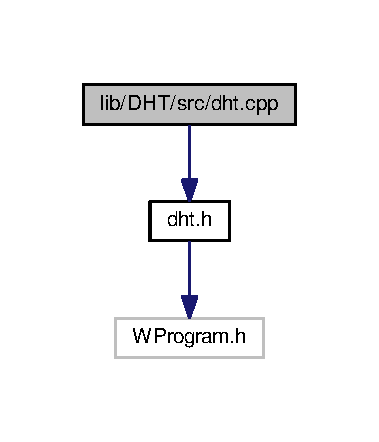
\includegraphics[width=182pt]{dht_8cpp__incl}
\end{center}
\end{figure}
\subsection*{Macros}
\begin{DoxyCompactItemize}
\item 
\#define \hyperlink{dht_8cpp_ae5d44a5fa9fd9d113f6bff639f06ddd6}{M\+I\+N\+\_\+\+I\+N\+T\+E\+R\+V\+AL}~2000
\end{DoxyCompactItemize}


\subsection{Macro Definition Documentation}
\index{dht.\+cpp@{dht.\+cpp}!M\+I\+N\+\_\+\+I\+N\+T\+E\+R\+V\+AL@{M\+I\+N\+\_\+\+I\+N\+T\+E\+R\+V\+AL}}
\index{M\+I\+N\+\_\+\+I\+N\+T\+E\+R\+V\+AL@{M\+I\+N\+\_\+\+I\+N\+T\+E\+R\+V\+AL}!dht.\+cpp@{dht.\+cpp}}
\subsubsection[{\texorpdfstring{M\+I\+N\+\_\+\+I\+N\+T\+E\+R\+V\+AL}{MIN_INTERVAL}}]{\setlength{\rightskip}{0pt plus 5cm}\#define M\+I\+N\+\_\+\+I\+N\+T\+E\+R\+V\+AL~2000}\hypertarget{dht_8cpp_ae5d44a5fa9fd9d113f6bff639f06ddd6}{}\label{dht_8cpp_ae5d44a5fa9fd9d113f6bff639f06ddd6}


Definition at line 9 of file dht.\+cpp.


\hypertarget{dht_8h}{}\section{lib/\+D\+H\+T/dht.h File Reference}
\label{dht_8h}\index{lib/\+D\+H\+T/dht.\+h@{lib/\+D\+H\+T/dht.\+h}}
{\ttfamily \#include $<$W\+Program.\+h$>$}\\*
{\ttfamily \#include $<$pins\+\_\+arduino.\+h$>$}\\*
Include dependency graph for dht.\+h\+:
% FIG 0
This graph shows which files directly or indirectly include this file\+:
% FIG 1
\subsection*{Classes}
\begin{DoxyCompactItemize}
\item 
class \hyperlink{classdht}{dht}
\end{DoxyCompactItemize}
\subsection*{Macros}
\begin{DoxyCompactItemize}
\item 
\#define \hyperlink{dht_8h_a981ffad927ef4f937207f4374cf33e1c}{D\+H\+T\+\_\+\+L\+I\+B\+\_\+\+V\+E\+R\+S\+I\+ON}~\char`\"{}0.\+1.\+21\char`\"{}
\item 
\#define \hyperlink{dht_8h_ab1b9cb0b80df3b9e1268f0e13ae80e11}{D\+H\+T\+L\+I\+B\+\_\+\+OK}~0
\item 
\#define \hyperlink{dht_8h_acda0653986ebb86e8bfed007bbf6a059}{D\+H\+T\+L\+I\+B\+\_\+\+E\+R\+R\+O\+R\+\_\+\+C\+H\+E\+C\+K\+S\+UM}~-\/1
\item 
\#define \hyperlink{dht_8h_ad6f86a85e5e1342005c23ceac36ec192}{D\+H\+T\+L\+I\+B\+\_\+\+E\+R\+R\+O\+R\+\_\+\+T\+I\+M\+E\+O\+UT}~-\/2
\item 
\#define \hyperlink{dht_8h_abc3e2e3759c80a2d31a059930990f49b}{D\+H\+T\+L\+I\+B\+\_\+\+E\+R\+R\+O\+R\+\_\+\+C\+O\+N\+N\+E\+CT}~-\/3
\item 
\#define \hyperlink{dht_8h_a6183db22278ba6596cd3d5aa26fb3b53}{D\+H\+T\+L\+I\+B\+\_\+\+E\+R\+R\+O\+R\+\_\+\+A\+C\+K\+\_\+L}~-\/4
\item 
\#define \hyperlink{dht_8h_adc68fb358de41083fe47747a8702cc35}{D\+H\+T\+L\+I\+B\+\_\+\+E\+R\+R\+O\+R\+\_\+\+A\+C\+K\+\_\+H}~-\/5
\item 
\#define \hyperlink{dht_8h_a5d7db73dafb20a282eb84d84778d3ee3}{D\+H\+T\+L\+I\+B\+\_\+\+D\+H\+T11\+\_\+\+W\+A\+K\+E\+UP}~18
\item 
\#define \hyperlink{dht_8h_ad4e4ae0f10e2d27eb4229474a55aadcb}{D\+H\+T\+L\+I\+B\+\_\+\+D\+H\+T\+\_\+\+W\+A\+K\+E\+UP}~1
\item 
\#define \hyperlink{dht_8h_a3715db703c7182b74af1d672b85e245b}{D\+H\+T\+L\+I\+B\+\_\+\+D\+H\+T11\+\_\+\+L\+E\+A\+D\+I\+N\+G\+\_\+\+Z\+E\+R\+OS}~1
\item 
\#define \hyperlink{dht_8h_a756c4be0b03863e3b04747e5fba12f87}{D\+H\+T\+L\+I\+B\+\_\+\+D\+H\+T\+\_\+\+L\+E\+A\+D\+I\+N\+G\+\_\+\+Z\+E\+R\+OS}~6
\item 
\#define \hyperlink{dht_8h_ad0e2e9ddfb66fe5e0727b63c7313ddf3}{D\+H\+T\+L\+I\+B\+\_\+\+T\+I\+M\+E\+O\+UT}~1000
\end{DoxyCompactItemize}


\subsection{Macro Definition Documentation}
\index{dht.\+h@{dht.\+h}!D\+H\+T\+\_\+\+L\+I\+B\+\_\+\+V\+E\+R\+S\+I\+ON@{D\+H\+T\+\_\+\+L\+I\+B\+\_\+\+V\+E\+R\+S\+I\+ON}}
\index{D\+H\+T\+\_\+\+L\+I\+B\+\_\+\+V\+E\+R\+S\+I\+ON@{D\+H\+T\+\_\+\+L\+I\+B\+\_\+\+V\+E\+R\+S\+I\+ON}!dht.\+h@{dht.\+h}}
\subsubsection[{\texorpdfstring{D\+H\+T\+\_\+\+L\+I\+B\+\_\+\+V\+E\+R\+S\+I\+ON}{DHT_LIB_VERSION}}]{\setlength{\rightskip}{0pt plus 5cm}\#define D\+H\+T\+\_\+\+L\+I\+B\+\_\+\+V\+E\+R\+S\+I\+ON~\char`\"{}0.\+1.\+21\char`\"{}}\hypertarget{dht_8h_a981ffad927ef4f937207f4374cf33e1c}{}\label{dht_8h_a981ffad927ef4f937207f4374cf33e1c}


Definition at line 22 of file dht.\+h.

\index{dht.\+h@{dht.\+h}!D\+H\+T\+L\+I\+B\+\_\+\+D\+H\+T11\+\_\+\+L\+E\+A\+D\+I\+N\+G\+\_\+\+Z\+E\+R\+OS@{D\+H\+T\+L\+I\+B\+\_\+\+D\+H\+T11\+\_\+\+L\+E\+A\+D\+I\+N\+G\+\_\+\+Z\+E\+R\+OS}}
\index{D\+H\+T\+L\+I\+B\+\_\+\+D\+H\+T11\+\_\+\+L\+E\+A\+D\+I\+N\+G\+\_\+\+Z\+E\+R\+OS@{D\+H\+T\+L\+I\+B\+\_\+\+D\+H\+T11\+\_\+\+L\+E\+A\+D\+I\+N\+G\+\_\+\+Z\+E\+R\+OS}!dht.\+h@{dht.\+h}}
\subsubsection[{\texorpdfstring{D\+H\+T\+L\+I\+B\+\_\+\+D\+H\+T11\+\_\+\+L\+E\+A\+D\+I\+N\+G\+\_\+\+Z\+E\+R\+OS}{DHTLIB_DHT11_LEADING_ZEROS}}]{\setlength{\rightskip}{0pt plus 5cm}\#define D\+H\+T\+L\+I\+B\+\_\+\+D\+H\+T11\+\_\+\+L\+E\+A\+D\+I\+N\+G\+\_\+\+Z\+E\+R\+OS~1}\hypertarget{dht_8h_a3715db703c7182b74af1d672b85e245b}{}\label{dht_8h_a3715db703c7182b74af1d672b85e245b}


Definition at line 34 of file dht.\+h.

\index{dht.\+h@{dht.\+h}!D\+H\+T\+L\+I\+B\+\_\+\+D\+H\+T11\+\_\+\+W\+A\+K\+E\+UP@{D\+H\+T\+L\+I\+B\+\_\+\+D\+H\+T11\+\_\+\+W\+A\+K\+E\+UP}}
\index{D\+H\+T\+L\+I\+B\+\_\+\+D\+H\+T11\+\_\+\+W\+A\+K\+E\+UP@{D\+H\+T\+L\+I\+B\+\_\+\+D\+H\+T11\+\_\+\+W\+A\+K\+E\+UP}!dht.\+h@{dht.\+h}}
\subsubsection[{\texorpdfstring{D\+H\+T\+L\+I\+B\+\_\+\+D\+H\+T11\+\_\+\+W\+A\+K\+E\+UP}{DHTLIB_DHT11_WAKEUP}}]{\setlength{\rightskip}{0pt plus 5cm}\#define D\+H\+T\+L\+I\+B\+\_\+\+D\+H\+T11\+\_\+\+W\+A\+K\+E\+UP~18}\hypertarget{dht_8h_a5d7db73dafb20a282eb84d84778d3ee3}{}\label{dht_8h_a5d7db73dafb20a282eb84d84778d3ee3}


Definition at line 31 of file dht.\+h.

\index{dht.\+h@{dht.\+h}!D\+H\+T\+L\+I\+B\+\_\+\+D\+H\+T\+\_\+\+L\+E\+A\+D\+I\+N\+G\+\_\+\+Z\+E\+R\+OS@{D\+H\+T\+L\+I\+B\+\_\+\+D\+H\+T\+\_\+\+L\+E\+A\+D\+I\+N\+G\+\_\+\+Z\+E\+R\+OS}}
\index{D\+H\+T\+L\+I\+B\+\_\+\+D\+H\+T\+\_\+\+L\+E\+A\+D\+I\+N\+G\+\_\+\+Z\+E\+R\+OS@{D\+H\+T\+L\+I\+B\+\_\+\+D\+H\+T\+\_\+\+L\+E\+A\+D\+I\+N\+G\+\_\+\+Z\+E\+R\+OS}!dht.\+h@{dht.\+h}}
\subsubsection[{\texorpdfstring{D\+H\+T\+L\+I\+B\+\_\+\+D\+H\+T\+\_\+\+L\+E\+A\+D\+I\+N\+G\+\_\+\+Z\+E\+R\+OS}{DHTLIB_DHT_LEADING_ZEROS}}]{\setlength{\rightskip}{0pt plus 5cm}\#define D\+H\+T\+L\+I\+B\+\_\+\+D\+H\+T\+\_\+\+L\+E\+A\+D\+I\+N\+G\+\_\+\+Z\+E\+R\+OS~6}\hypertarget{dht_8h_a756c4be0b03863e3b04747e5fba12f87}{}\label{dht_8h_a756c4be0b03863e3b04747e5fba12f87}


Definition at line 35 of file dht.\+h.

\index{dht.\+h@{dht.\+h}!D\+H\+T\+L\+I\+B\+\_\+\+D\+H\+T\+\_\+\+W\+A\+K\+E\+UP@{D\+H\+T\+L\+I\+B\+\_\+\+D\+H\+T\+\_\+\+W\+A\+K\+E\+UP}}
\index{D\+H\+T\+L\+I\+B\+\_\+\+D\+H\+T\+\_\+\+W\+A\+K\+E\+UP@{D\+H\+T\+L\+I\+B\+\_\+\+D\+H\+T\+\_\+\+W\+A\+K\+E\+UP}!dht.\+h@{dht.\+h}}
\subsubsection[{\texorpdfstring{D\+H\+T\+L\+I\+B\+\_\+\+D\+H\+T\+\_\+\+W\+A\+K\+E\+UP}{DHTLIB_DHT_WAKEUP}}]{\setlength{\rightskip}{0pt plus 5cm}\#define D\+H\+T\+L\+I\+B\+\_\+\+D\+H\+T\+\_\+\+W\+A\+K\+E\+UP~1}\hypertarget{dht_8h_ad4e4ae0f10e2d27eb4229474a55aadcb}{}\label{dht_8h_ad4e4ae0f10e2d27eb4229474a55aadcb}


Definition at line 32 of file dht.\+h.

\index{dht.\+h@{dht.\+h}!D\+H\+T\+L\+I\+B\+\_\+\+E\+R\+R\+O\+R\+\_\+\+A\+C\+K\+\_\+H@{D\+H\+T\+L\+I\+B\+\_\+\+E\+R\+R\+O\+R\+\_\+\+A\+C\+K\+\_\+H}}
\index{D\+H\+T\+L\+I\+B\+\_\+\+E\+R\+R\+O\+R\+\_\+\+A\+C\+K\+\_\+H@{D\+H\+T\+L\+I\+B\+\_\+\+E\+R\+R\+O\+R\+\_\+\+A\+C\+K\+\_\+H}!dht.\+h@{dht.\+h}}
\subsubsection[{\texorpdfstring{D\+H\+T\+L\+I\+B\+\_\+\+E\+R\+R\+O\+R\+\_\+\+A\+C\+K\+\_\+H}{DHTLIB_ERROR_ACK_H}}]{\setlength{\rightskip}{0pt plus 5cm}\#define D\+H\+T\+L\+I\+B\+\_\+\+E\+R\+R\+O\+R\+\_\+\+A\+C\+K\+\_\+H~-\/5}\hypertarget{dht_8h_adc68fb358de41083fe47747a8702cc35}{}\label{dht_8h_adc68fb358de41083fe47747a8702cc35}


Definition at line 29 of file dht.\+h.

\index{dht.\+h@{dht.\+h}!D\+H\+T\+L\+I\+B\+\_\+\+E\+R\+R\+O\+R\+\_\+\+A\+C\+K\+\_\+L@{D\+H\+T\+L\+I\+B\+\_\+\+E\+R\+R\+O\+R\+\_\+\+A\+C\+K\+\_\+L}}
\index{D\+H\+T\+L\+I\+B\+\_\+\+E\+R\+R\+O\+R\+\_\+\+A\+C\+K\+\_\+L@{D\+H\+T\+L\+I\+B\+\_\+\+E\+R\+R\+O\+R\+\_\+\+A\+C\+K\+\_\+L}!dht.\+h@{dht.\+h}}
\subsubsection[{\texorpdfstring{D\+H\+T\+L\+I\+B\+\_\+\+E\+R\+R\+O\+R\+\_\+\+A\+C\+K\+\_\+L}{DHTLIB_ERROR_ACK_L}}]{\setlength{\rightskip}{0pt plus 5cm}\#define D\+H\+T\+L\+I\+B\+\_\+\+E\+R\+R\+O\+R\+\_\+\+A\+C\+K\+\_\+L~-\/4}\hypertarget{dht_8h_a6183db22278ba6596cd3d5aa26fb3b53}{}\label{dht_8h_a6183db22278ba6596cd3d5aa26fb3b53}


Definition at line 28 of file dht.\+h.

\index{dht.\+h@{dht.\+h}!D\+H\+T\+L\+I\+B\+\_\+\+E\+R\+R\+O\+R\+\_\+\+C\+H\+E\+C\+K\+S\+UM@{D\+H\+T\+L\+I\+B\+\_\+\+E\+R\+R\+O\+R\+\_\+\+C\+H\+E\+C\+K\+S\+UM}}
\index{D\+H\+T\+L\+I\+B\+\_\+\+E\+R\+R\+O\+R\+\_\+\+C\+H\+E\+C\+K\+S\+UM@{D\+H\+T\+L\+I\+B\+\_\+\+E\+R\+R\+O\+R\+\_\+\+C\+H\+E\+C\+K\+S\+UM}!dht.\+h@{dht.\+h}}
\subsubsection[{\texorpdfstring{D\+H\+T\+L\+I\+B\+\_\+\+E\+R\+R\+O\+R\+\_\+\+C\+H\+E\+C\+K\+S\+UM}{DHTLIB_ERROR_CHECKSUM}}]{\setlength{\rightskip}{0pt plus 5cm}\#define D\+H\+T\+L\+I\+B\+\_\+\+E\+R\+R\+O\+R\+\_\+\+C\+H\+E\+C\+K\+S\+UM~-\/1}\hypertarget{dht_8h_acda0653986ebb86e8bfed007bbf6a059}{}\label{dht_8h_acda0653986ebb86e8bfed007bbf6a059}


Definition at line 25 of file dht.\+h.

\index{dht.\+h@{dht.\+h}!D\+H\+T\+L\+I\+B\+\_\+\+E\+R\+R\+O\+R\+\_\+\+C\+O\+N\+N\+E\+CT@{D\+H\+T\+L\+I\+B\+\_\+\+E\+R\+R\+O\+R\+\_\+\+C\+O\+N\+N\+E\+CT}}
\index{D\+H\+T\+L\+I\+B\+\_\+\+E\+R\+R\+O\+R\+\_\+\+C\+O\+N\+N\+E\+CT@{D\+H\+T\+L\+I\+B\+\_\+\+E\+R\+R\+O\+R\+\_\+\+C\+O\+N\+N\+E\+CT}!dht.\+h@{dht.\+h}}
\subsubsection[{\texorpdfstring{D\+H\+T\+L\+I\+B\+\_\+\+E\+R\+R\+O\+R\+\_\+\+C\+O\+N\+N\+E\+CT}{DHTLIB_ERROR_CONNECT}}]{\setlength{\rightskip}{0pt plus 5cm}\#define D\+H\+T\+L\+I\+B\+\_\+\+E\+R\+R\+O\+R\+\_\+\+C\+O\+N\+N\+E\+CT~-\/3}\hypertarget{dht_8h_abc3e2e3759c80a2d31a059930990f49b}{}\label{dht_8h_abc3e2e3759c80a2d31a059930990f49b}


Definition at line 27 of file dht.\+h.

\index{dht.\+h@{dht.\+h}!D\+H\+T\+L\+I\+B\+\_\+\+E\+R\+R\+O\+R\+\_\+\+T\+I\+M\+E\+O\+UT@{D\+H\+T\+L\+I\+B\+\_\+\+E\+R\+R\+O\+R\+\_\+\+T\+I\+M\+E\+O\+UT}}
\index{D\+H\+T\+L\+I\+B\+\_\+\+E\+R\+R\+O\+R\+\_\+\+T\+I\+M\+E\+O\+UT@{D\+H\+T\+L\+I\+B\+\_\+\+E\+R\+R\+O\+R\+\_\+\+T\+I\+M\+E\+O\+UT}!dht.\+h@{dht.\+h}}
\subsubsection[{\texorpdfstring{D\+H\+T\+L\+I\+B\+\_\+\+E\+R\+R\+O\+R\+\_\+\+T\+I\+M\+E\+O\+UT}{DHTLIB_ERROR_TIMEOUT}}]{\setlength{\rightskip}{0pt plus 5cm}\#define D\+H\+T\+L\+I\+B\+\_\+\+E\+R\+R\+O\+R\+\_\+\+T\+I\+M\+E\+O\+UT~-\/2}\hypertarget{dht_8h_ad6f86a85e5e1342005c23ceac36ec192}{}\label{dht_8h_ad6f86a85e5e1342005c23ceac36ec192}


Definition at line 26 of file dht.\+h.

\index{dht.\+h@{dht.\+h}!D\+H\+T\+L\+I\+B\+\_\+\+OK@{D\+H\+T\+L\+I\+B\+\_\+\+OK}}
\index{D\+H\+T\+L\+I\+B\+\_\+\+OK@{D\+H\+T\+L\+I\+B\+\_\+\+OK}!dht.\+h@{dht.\+h}}
\subsubsection[{\texorpdfstring{D\+H\+T\+L\+I\+B\+\_\+\+OK}{DHTLIB_OK}}]{\setlength{\rightskip}{0pt plus 5cm}\#define D\+H\+T\+L\+I\+B\+\_\+\+OK~0}\hypertarget{dht_8h_ab1b9cb0b80df3b9e1268f0e13ae80e11}{}\label{dht_8h_ab1b9cb0b80df3b9e1268f0e13ae80e11}


Definition at line 24 of file dht.\+h.

\index{dht.\+h@{dht.\+h}!D\+H\+T\+L\+I\+B\+\_\+\+T\+I\+M\+E\+O\+UT@{D\+H\+T\+L\+I\+B\+\_\+\+T\+I\+M\+E\+O\+UT}}
\index{D\+H\+T\+L\+I\+B\+\_\+\+T\+I\+M\+E\+O\+UT@{D\+H\+T\+L\+I\+B\+\_\+\+T\+I\+M\+E\+O\+UT}!dht.\+h@{dht.\+h}}
\subsubsection[{\texorpdfstring{D\+H\+T\+L\+I\+B\+\_\+\+T\+I\+M\+E\+O\+UT}{DHTLIB_TIMEOUT}}]{\setlength{\rightskip}{0pt plus 5cm}\#define D\+H\+T\+L\+I\+B\+\_\+\+T\+I\+M\+E\+O\+UT~1000}\hypertarget{dht_8h_ad0e2e9ddfb66fe5e0727b63c7313ddf3}{}\label{dht_8h_ad0e2e9ddfb66fe5e0727b63c7313ddf3}


Definition at line 43 of file dht.\+h.


\hypertarget{ldr_8cpp}{}\section{lib/\+L\+D\+R/src/ldr.cpp File Reference}
\label{ldr_8cpp}\index{lib/\+L\+D\+R/src/ldr.\+cpp@{lib/\+L\+D\+R/src/ldr.\+cpp}}
{\ttfamily \#include $<$Arduino.\+h$>$}\\*
{\ttfamily \#include \char`\"{}ldr.\+hpp\char`\"{}}\\*
Include dependency graph for ldr.\+cpp\+:\nopagebreak
\begin{figure}[H]
\begin{center}
\leavevmode
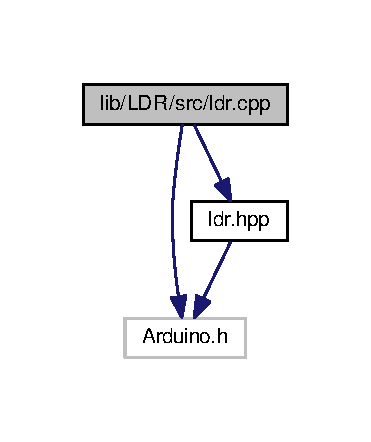
\includegraphics[width=178pt]{ldr_8cpp__incl}
\end{center}
\end{figure}

\hypertarget{ldr_8hpp}{}\section{lib/\+L\+D\+R/src/ldr.hpp File Reference}
\label{ldr_8hpp}\index{lib/\+L\+D\+R/src/ldr.\+hpp@{lib/\+L\+D\+R/src/ldr.\+hpp}}
{\ttfamily \#include $<$Arduino.\+h$>$}\\*
Include dependency graph for ldr.\+hpp\+:
% FIG 0
This graph shows which files directly or indirectly include this file\+:
% FIG 1
\subsection*{Classes}
\begin{DoxyCompactItemize}
\item 
class \hyperlink{classldr}{ldr}
\end{DoxyCompactItemize}

\hypertarget{_m_q_sensor_8cpp}{}\section{lib/\+M\+Q-\/\+Sensor/src/\+M\+Q\+Sensor.cpp File Reference}
\label{_m_q_sensor_8cpp}\index{lib/\+M\+Q-\/\+Sensor/src/\+M\+Q\+Sensor.\+cpp@{lib/\+M\+Q-\/\+Sensor/src/\+M\+Q\+Sensor.\+cpp}}
{\ttfamily \#include $<$Arduino.\+h$>$}\\*
{\ttfamily \#include \char`\"{}M\+Q\+Sensor.\+hpp\char`\"{}}\\*
Include dependency graph for M\+Q\+Sensor.\+cpp\+:\nopagebreak
\begin{figure}[H]
\begin{center}
\leavevmode
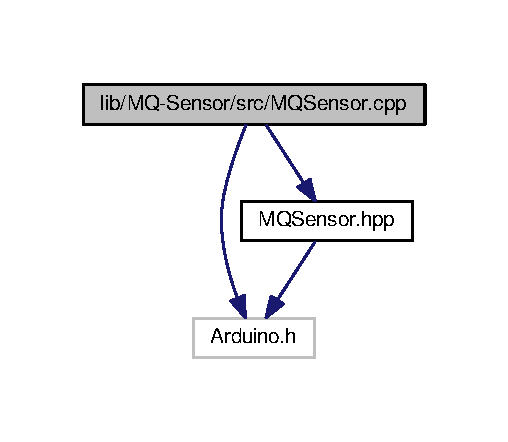
\includegraphics[width=244pt]{_m_q_sensor_8cpp__incl}
\end{center}
\end{figure}
\subsection*{Functions}
\begin{DoxyCompactItemize}
\item 
{\footnotesize template$<$typename T $>$ }\\T \hyperlink{_m_q_sensor_8cpp_a93e58338e8b2c1f572bbcccb7eff9714}{map} (T x, T in\+\_\+min, T in\+\_\+max, T out\+\_\+min, T out\+\_\+max)
\end{DoxyCompactItemize}


\subsection{Function Documentation}
\index{M\+Q\+Sensor.\+cpp@{M\+Q\+Sensor.\+cpp}!map@{map}}
\index{map@{map}!M\+Q\+Sensor.\+cpp@{M\+Q\+Sensor.\+cpp}}
\subsubsection[{\texorpdfstring{map(\+T x, T in\+\_\+min, T in\+\_\+max, T out\+\_\+min, T out\+\_\+max)}{map(T x, T in_min, T in_max, T out_min, T out_max)}}]{\setlength{\rightskip}{0pt plus 5cm}template$<$typename T $>$ T map (
\begin{DoxyParamCaption}
\item[{T}]{x, }
\item[{T}]{in\+\_\+min, }
\item[{T}]{in\+\_\+max, }
\item[{T}]{out\+\_\+min, }
\item[{T}]{out\+\_\+max}
\end{DoxyParamCaption}
)}\hypertarget{_m_q_sensor_8cpp_a93e58338e8b2c1f572bbcccb7eff9714}{}\label{_m_q_sensor_8cpp_a93e58338e8b2c1f572bbcccb7eff9714}
Re-\/maps a number from one range to another. That is, a value of in\+\_\+min would get mapped to out\+\_\+min, a value of in\+\_\+max to out\+\_\+max, values in-\/between to values in-\/between, etc. 
\begin{DoxyParams}{Parameters}
{\em x} & The value to be mapped. \\
\hline
{\em in\+\_\+min} & The lower bond of the value\textquotesingle{}s current range. \\
\hline
{\em in\+\_\+max} & The upper bond of the value\textquotesingle{}s current range. \\
\hline
{\em out\+\_\+min} & The lower bond of the value\textquotesingle{}s target range. \\
\hline
{\em out\+\_\+max} & The upper bond of the value\textquotesingle{}s target range. \\
\hline
\end{DoxyParams}
\begin{DoxyReturn}{Returns}
The mapped value. 
\end{DoxyReturn}


Definition at line 26 of file M\+Q\+Sensor.\+cpp.


\hypertarget{_m_q_sensor_8hpp}{}\section{lib/\+M\+Q-\/\+Sensor/src/\+M\+Q\+Sensor.hpp File Reference}
\label{_m_q_sensor_8hpp}\index{lib/\+M\+Q-\/\+Sensor/src/\+M\+Q\+Sensor.\+hpp@{lib/\+M\+Q-\/\+Sensor/src/\+M\+Q\+Sensor.\+hpp}}
{\ttfamily \#include $<$Arduino.\+h$>$}\\*
Include dependency graph for M\+Q\+Sensor.\+hpp\+:\nopagebreak
\begin{figure}[H]
\begin{center}
\leavevmode
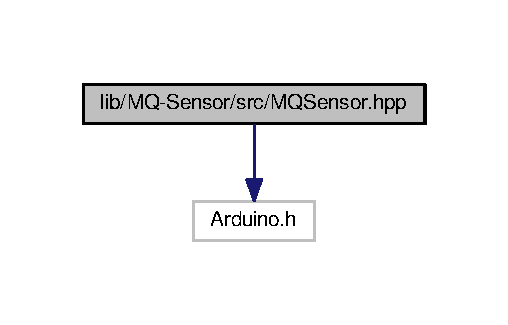
\includegraphics[width=244pt]{_m_q_sensor_8hpp__incl}
\end{center}
\end{figure}
This graph shows which files directly or indirectly include this file\+:\nopagebreak
\begin{figure}[H]
\begin{center}
\leavevmode
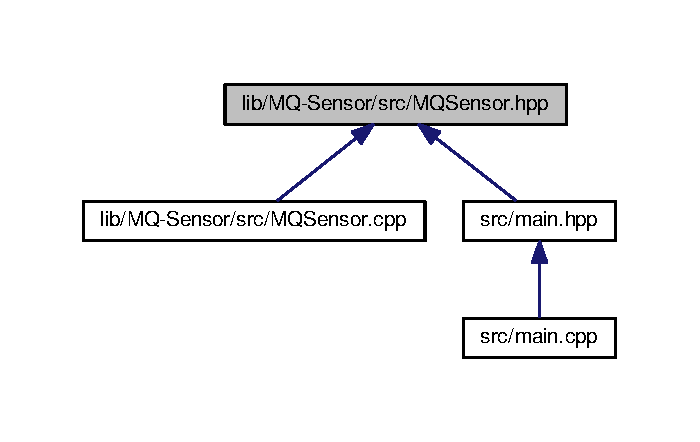
\includegraphics[width=336pt]{_m_q_sensor_8hpp__dep__incl}
\end{center}
\end{figure}
\subsection*{Classes}
\begin{DoxyCompactItemize}
\item 
class \hyperlink{class_m_q_sensor}{M\+Q\+Sensor}
\item 
class \hyperlink{class_m_q_dummy}{M\+Q\+Dummy}
\item 
class \hyperlink{class_m_q_potentiometer}{M\+Q\+Potentiometer}
\item 
class \hyperlink{class_m_q3}{M\+Q3}
\item 
class \hyperlink{class_m_q7}{M\+Q7}
\end{DoxyCompactItemize}
\subsection*{Enumerations}
\begin{DoxyCompactItemize}
\item 
enum \hyperlink{_m_q_sensor_8hpp_aa39cce9d2f2c6464e774b8f5684bd664}{S\+E\+N\+S\+O\+R\+\_\+\+T\+Y\+PE} \+: const uint8\+\_\+t 
\item 
enum \hyperlink{_m_q_sensor_8hpp_adc1ba5bd8d887ddb6973cff15d9a1501}{G\+A\+S\+\_\+\+T\+Y\+PE} \+: const uint8\+\_\+t 
\end{DoxyCompactItemize}


\subsection{Enumeration Type Documentation}
\index{M\+Q\+Sensor.\+hpp@{M\+Q\+Sensor.\+hpp}!G\+A\+S\+\_\+\+T\+Y\+PE@{G\+A\+S\+\_\+\+T\+Y\+PE}}
\index{G\+A\+S\+\_\+\+T\+Y\+PE@{G\+A\+S\+\_\+\+T\+Y\+PE}!M\+Q\+Sensor.\+hpp@{M\+Q\+Sensor.\+hpp}}
\subsubsection[{\texorpdfstring{G\+A\+S\+\_\+\+T\+Y\+PE}{GAS_TYPE}}]{\setlength{\rightskip}{0pt plus 5cm}enum {\bf G\+A\+S\+\_\+\+T\+Y\+PE} \+: const uint8\+\_\+t}\hypertarget{_m_q_sensor_8hpp_adc1ba5bd8d887ddb6973cff15d9a1501}{}\label{_m_q_sensor_8hpp_adc1ba5bd8d887ddb6973cff15d9a1501}


Definition at line 29 of file M\+Q\+Sensor.\+hpp.

\index{M\+Q\+Sensor.\+hpp@{M\+Q\+Sensor.\+hpp}!S\+E\+N\+S\+O\+R\+\_\+\+T\+Y\+PE@{S\+E\+N\+S\+O\+R\+\_\+\+T\+Y\+PE}}
\index{S\+E\+N\+S\+O\+R\+\_\+\+T\+Y\+PE@{S\+E\+N\+S\+O\+R\+\_\+\+T\+Y\+PE}!M\+Q\+Sensor.\+hpp@{M\+Q\+Sensor.\+hpp}}
\subsubsection[{\texorpdfstring{S\+E\+N\+S\+O\+R\+\_\+\+T\+Y\+PE}{SENSOR_TYPE}}]{\setlength{\rightskip}{0pt plus 5cm}enum {\bf S\+E\+N\+S\+O\+R\+\_\+\+T\+Y\+PE} \+: const uint8\+\_\+t}\hypertarget{_m_q_sensor_8hpp_aa39cce9d2f2c6464e774b8f5684bd664}{}\label{_m_q_sensor_8hpp_aa39cce9d2f2c6464e774b8f5684bd664}


Definition at line 15 of file M\+Q\+Sensor.\+hpp.


\hypertarget{old_2_print_manager_8cpp}{}\section{lib/\+Print\+Manager/old/\+Print\+Manager.cpp File Reference}
\label{old_2_print_manager_8cpp}\index{lib/\+Print\+Manager/old/\+Print\+Manager.\+cpp@{lib/\+Print\+Manager/old/\+Print\+Manager.\+cpp}}
{\ttfamily \#include $<$Arduino.\+h$>$}\\*
{\ttfamily \#include \char`\"{}Print\+Manager.\+hpp\char`\"{}}\\*
Include dependency graph for Print\+Manager.\+cpp\+:
% FIG 0

\hypertarget{src_2_print_manager_8cpp}{}\section{lib/\+Print\+Manager/src/\+Print\+Manager.cpp File Reference}
\label{src_2_print_manager_8cpp}\index{lib/\+Print\+Manager/src/\+Print\+Manager.\+cpp@{lib/\+Print\+Manager/src/\+Print\+Manager.\+cpp}}
{\ttfamily \#include $<$Arduino.\+h$>$}\\*
{\ttfamily \#include \char`\"{}Print\+Manager.\+hpp\char`\"{}}\\*
Include dependency graph for Print\+Manager.\+cpp\+:
% FIG 0
\subsection*{Functions}
\begin{DoxyCompactItemize}
\item 
constexpr int \hyperlink{src_2_print_manager_8cpp_ac56103e1cb66ddb548cc87fa00e0e0c7}{to\+Int} (const char c)
\end{DoxyCompactItemize}


\subsection{Function Documentation}
\index{src/\+Print\+Manager.\+cpp@{src/\+Print\+Manager.\+cpp}!to\+Int@{to\+Int}}
\index{to\+Int@{to\+Int}!src/\+Print\+Manager.\+cpp@{src/\+Print\+Manager.\+cpp}}
\subsubsection[{\texorpdfstring{to\+Int(const char c)}{toInt(const char c)}}]{\setlength{\rightskip}{0pt plus 5cm}constexpr int to\+Int (
\begin{DoxyParamCaption}
\item[{const char}]{c}
\end{DoxyParamCaption}
)}\hypertarget{src_2_print_manager_8cpp_ac56103e1cb66ddb548cc87fa00e0e0c7}{}\label{src_2_print_manager_8cpp_ac56103e1cb66ddb548cc87fa00e0e0c7}


Definition at line 4 of file Print\+Manager.\+cpp.


\hypertarget{old_2_print_manager_8hpp}{}\section{lib/\+Print\+Manager/old/\+Print\+Manager.hpp File Reference}
\label{old_2_print_manager_8hpp}\index{lib/\+Print\+Manager/old/\+Print\+Manager.\+hpp@{lib/\+Print\+Manager/old/\+Print\+Manager.\+hpp}}
{\ttfamily \#include $<$Arduino.\+h$>$}\\*
Include dependency graph for Print\+Manager.\+hpp\+:
% FIG 0
This graph shows which files directly or indirectly include this file\+:
% FIG 1
\subsection*{Classes}
\begin{DoxyCompactItemize}
\item 
class \hyperlink{class_print_manager}{Print\+Manager}
\end{DoxyCompactItemize}

\hypertarget{src_2_print_manager_8hpp}{}\section{lib/\+Print\+Manager/src/\+Print\+Manager.hpp File Reference}
\label{src_2_print_manager_8hpp}\index{lib/\+Print\+Manager/src/\+Print\+Manager.\+hpp@{lib/\+Print\+Manager/src/\+Print\+Manager.\+hpp}}
{\ttfamily \#include $<$Arduino.\+h$>$}\\*
{\ttfamily \#include $<$Software\+Serial.\+h$>$}\\*
Include dependency graph for Print\+Manager.\+hpp\+:
% FIG 0
This graph shows which files directly or indirectly include this file\+:
% FIG 1
\subsection*{Classes}
\begin{DoxyCompactItemize}
\item 
class \hyperlink{class_print_manager}{Print\+Manager}
\end{DoxyCompactItemize}
\subsection*{Enumerations}
\begin{DoxyCompactItemize}
\item 
enum \hyperlink{src_2_print_manager_8hpp_ac4250c605bd199b412d7419ad514699f}{serial\+Port\+Type} \+: const uint8\+\_\+t 
\end{DoxyCompactItemize}


\subsection{Enumeration Type Documentation}
\index{src/\+Print\+Manager.\+hpp@{src/\+Print\+Manager.\+hpp}!serial\+Port\+Type@{serial\+Port\+Type}}
\index{serial\+Port\+Type@{serial\+Port\+Type}!src/\+Print\+Manager.\+hpp@{src/\+Print\+Manager.\+hpp}}
\subsubsection[{\texorpdfstring{serial\+Port\+Type}{serialPortType}}]{\setlength{\rightskip}{0pt plus 5cm}enum {\bf serial\+Port\+Type} \+: const uint8\+\_\+t}\hypertarget{src_2_print_manager_8hpp_ac4250c605bd199b412d7419ad514699f}{}\label{src_2_print_manager_8hpp_ac4250c605bd199b412d7419ad514699f}


Definition at line 8 of file Print\+Manager.\+hpp.


\hypertarget{_r_e_a_d_m_e_8md}{}\section{R\+E\+A\+D\+M\+E.\+md File Reference}
\label{_r_e_a_d_m_e_8md}\index{R\+E\+A\+D\+M\+E.\+md@{R\+E\+A\+D\+M\+E.\+md}}

\hypertarget{_r_e_a_d_m_e___p_t_b_r_8md}{}\section{R\+E\+A\+D\+M\+E\+\_\+\+P\+T\+B\+R.\+md File Reference}
\label{_r_e_a_d_m_e___p_t_b_r_8md}\index{R\+E\+A\+D\+M\+E\+\_\+\+P\+T\+B\+R.\+md@{R\+E\+A\+D\+M\+E\+\_\+\+P\+T\+B\+R.\+md}}

\hypertarget{main_8cpp}{}\section{src/main.cpp File Reference}
\label{main_8cpp}\index{src/main.\+cpp@{src/main.\+cpp}}
{\ttfamily \#include \char`\"{}Arduino.\+h\char`\"{}}\\*
{\ttfamily \#include \char`\"{}main.\+hpp\char`\"{}}\\*
Include dependency graph for main.\+cpp\+:\nopagebreak
\begin{figure}[H]
\begin{center}
\leavevmode
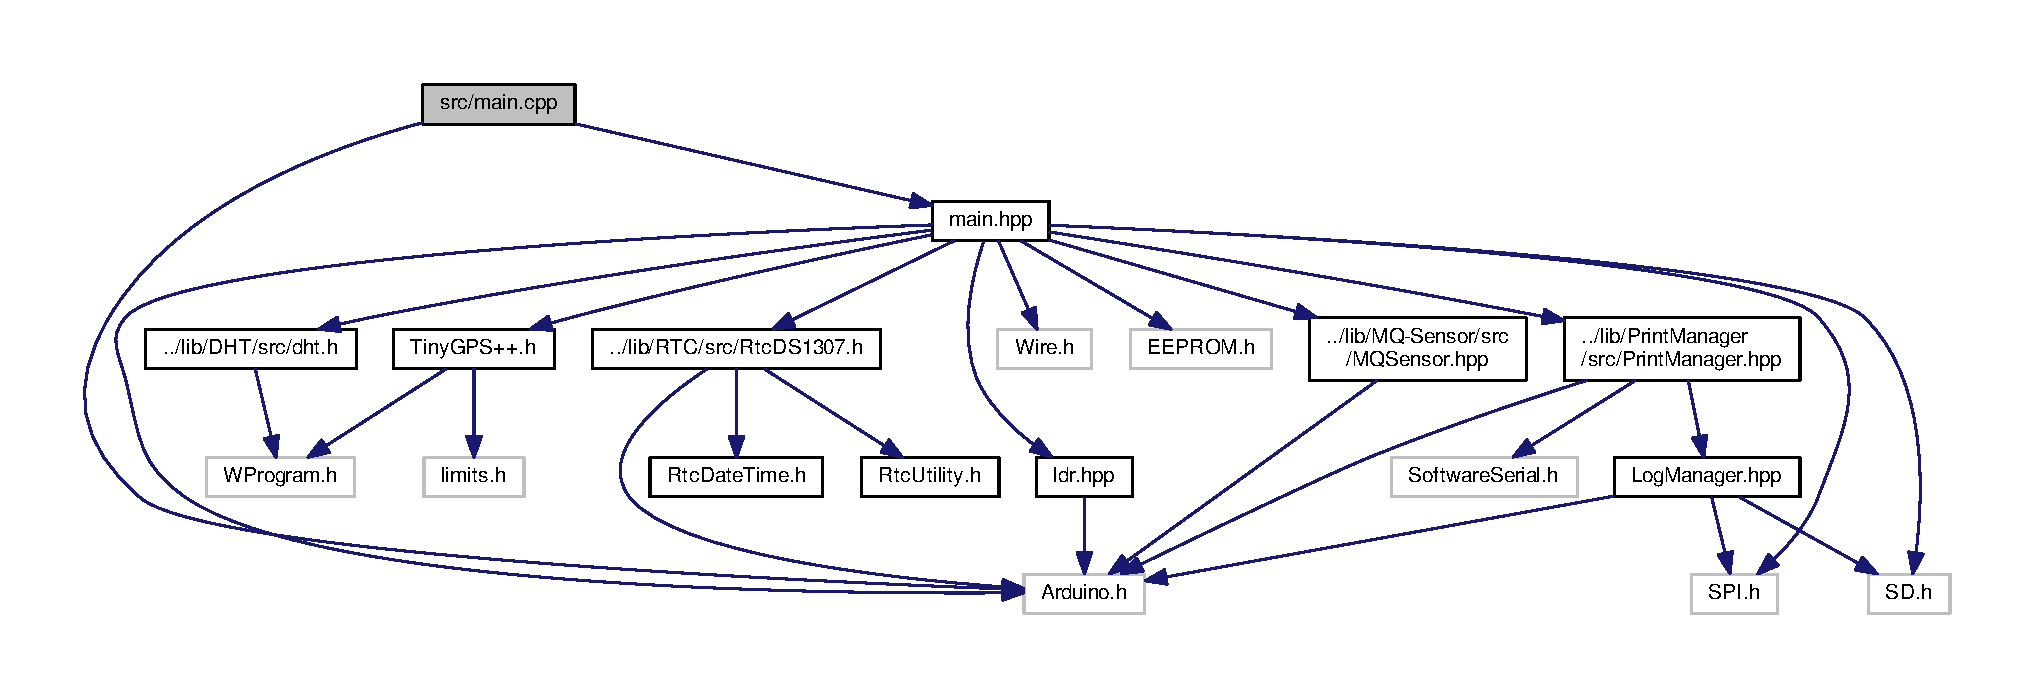
\includegraphics[width=350pt]{main_8cpp__incl}
\end{center}
\end{figure}
\subsection*{Functions}
\begin{DoxyCompactItemize}
\item 
void \hyperlink{main_8cpp_a4fc01d736fe50cf5b977f755b675f11d}{setup} ()
\item 
void \hyperlink{main_8cpp_afe461d27b9c48d5921c00d521181f12f}{loop} ()
\end{DoxyCompactItemize}


\subsection{Function Documentation}
\index{main.\+cpp@{main.\+cpp}!loop@{loop}}
\index{loop@{loop}!main.\+cpp@{main.\+cpp}}
\subsubsection[{\texorpdfstring{loop()}{loop()}}]{\setlength{\rightskip}{0pt plus 5cm}void loop (
\begin{DoxyParamCaption}
{}
\end{DoxyParamCaption}
)}\hypertarget{main_8cpp_afe461d27b9c48d5921c00d521181f12f}{}\label{main_8cpp_afe461d27b9c48d5921c00d521181f12f}


Definition at line 70 of file main.\+cpp.

\index{main.\+cpp@{main.\+cpp}!setup@{setup}}
\index{setup@{setup}!main.\+cpp@{main.\+cpp}}
\subsubsection[{\texorpdfstring{setup()}{setup()}}]{\setlength{\rightskip}{0pt plus 5cm}void setup (
\begin{DoxyParamCaption}
{}
\end{DoxyParamCaption}
)}\hypertarget{main_8cpp_a4fc01d736fe50cf5b977f755b675f11d}{}\label{main_8cpp_a4fc01d736fe50cf5b977f755b675f11d}


Definition at line 18 of file main.\+cpp.


\hypertarget{main_8hpp}{}\section{src/main.hpp File Reference}
\label{main_8hpp}\index{src/main.\+hpp@{src/main.\+hpp}}
{\ttfamily \#include \char`\"{}Arduino.\+h\char`\"{}}\\*
{\ttfamily \#include \char`\"{}dht.\+h\char`\"{}}\\*
Include dependency graph for main.\+hpp\+:
% FIG 0
This graph shows which files directly or indirectly include this file\+:
% FIG 1
\subsection*{Functions}
\begin{DoxyCompactItemize}
\item 
void \hyperlink{main_8hpp_a4a303c3b1de7cf54a8a5b31232355f74}{dht\+Debug} (\hyperlink{classdht}{dht} Sensor, uint8\+\_\+t \hyperlink{main_8cpp_a79111e78831efb8ac76fa8123357475e}{D\+H\+T11\+\_\+\+P\+IN})
\end{DoxyCompactItemize}


\subsection{Function Documentation}
\index{main.\+hpp@{main.\+hpp}!dht\+Debug@{dht\+Debug}}
\index{dht\+Debug@{dht\+Debug}!main.\+hpp@{main.\+hpp}}
\subsubsection[{\texorpdfstring{dht\+Debug(dht Sensor, uint8\+\_\+t D\+H\+T11\+\_\+\+P\+I\+N)}{dhtDebug(dht Sensor, uint8_t DHT11_PIN)}}]{\setlength{\rightskip}{0pt plus 5cm}void dht\+Debug (
\begin{DoxyParamCaption}
\item[{{\bf dht}}]{Sensor, }
\item[{uint8\+\_\+t}]{D\+H\+T11\+\_\+\+P\+IN}
\end{DoxyParamCaption}
)}\hypertarget{main_8hpp_a4a303c3b1de7cf54a8a5b31232355f74}{}\label{main_8hpp_a4a303c3b1de7cf54a8a5b31232355f74}


Definition at line 8 of file main.\+hpp.



Here is the call graph for this function\+:
% FIG 2




Here is the caller graph for this function\+:
% FIG 3



%--- End generated contents ---

% Index
\backmatter
\newpage
\phantomsection
\clearemptydoublepage
\addcontentsline{toc}{chapter}{Index}
\printindex

\end{document}
